%!TEX root = ../dissertation.tex
\chapter{Algorithms}
\label{chap:algos}

The problems of atomic norm decomposition and regularization have linear and
quadratic objectives, and can be efficiently be optimized provided there is an
efficient way to test membership in the constraint sets. The constraint sets of
the primal and dual problems are the sublevel sets of the atomic and the dual
atomic norm. Therefore, it is sufficient to develop efficient characterizations
of the atomic norm ball.

For the special case of Fourier measurements, the atomic norm ball has
semidefinite characterizations which we derive in this chapter. The positive
case is classical and comes from moment theory and the dual theory of positive
polynomials. We will review the results for the positive case and provide the
proofs for completeness. We will also derive the semidefinite characterization
for the more general complex case using these results. We provide a reasonably
fast method for solving this SDP via the Alternating Direction Method of
Multipliers (ADMM)~\cite{BertsekasParallelBook,admm2011}. Our ADMM
implementation can solve instances with a thousand observations in a few
minutes.

While the SDP based AST algorithm can be thought of as solving an infinite
dimensional Lasso problem, the computational complexity can be prohibitive for
very large instances. To compensate, we show that solving the Lasso problem on
an oversampled grid of frequencies approximates the solution of the atomic norm
minimization problem to a resolution sufficiently high to guarantee excellent
mean-squared error (MSE). The gridded problem reduces to the Lasso, and by
leveraging the Fast Fourier Transform (FFT), can be rapidly solved with freely
available software such as SpaRSA~\cite{wright09}. A Lasso problem with
thousands of observations can be solved in under a second using Matlab on a
laptop. The prediction error and the localization accuracy for line spectral
estimation both increase as the oversampling factor increases, even if the
actual set of frequencies in the line spectral signal are off the Lasso grid.

For the problem of system identification, there are no tractable semidefinite
formulations. While it is possible to develop a sequence of semidefinite
relaxations, we instead describe how we can use a discretization approach for
the atomic soft thresholding (AST) problem described in Chapter~\ref{chap:ast}
and this essentially reduces to solving a Lasso problem on an overcomplete grid.
Our proofs for discretized atomic soft thresholding (DAST) demonstrate why Lasso
is often successful even for off-grid data.

In this chapter, we also collect our experimental results using these algorithms
on Line Spectral Signals. We compare and contrast our algorithms, AST and Lasso,
with classical line spectral algorithms including MUSIC~\cite{music},and
Cadzow's ~\cite{cadzow02} and Matrix Pencil~\cite{hua02} methods . Our
experiments indicate that both AST and the Lasso approximation outperform
classical methods in low SNR even when we provide the exact model order to the
classical approaches. Moreover, AST has the same complexity as Cadzow's method,
alternating between a least-squares step and an eigenvalue thresholding step.
The discretized Lasso-based algorithm has even lower computational complexity,
consisting of iterations based upon the FFT and simple linear time
soft-thresholding.



\subsection*{Summary and Organization of this chapter} % (fold)
\label{sub:main_results}
Our goal in this chapter is to develop an algorithm to solve the Atomic Soft
Thresholding (AST) problem, defined in Chapter~\ref{chap:ast}:
\begin{align}
\begin{split}
\minimize_x & \frac{1}{2}\vnorm{y-x}_2^2 + \tau \vnorm{x}_\A,
\end{split}	
\end{align}
and its corresponding dual problem:
\begin{align}
\begin{split}
\maximize_x & \frac{1}{2}\left(\vnorm{y}_2^2 - \vnorm{y-\tau q}_2^2\right)\\
\text{subject to } & \vnorm{q}_\A^* \leq 1. 
\end{split}
\end{align}
For certain atomic sets, we can compute the atomic norms efficiently. We will
develop computable characterizations of the atomic norm and its dual for line
spectral atomic sets defined in Chapter~\ref{chap:linespect}. First, let us
recall the definition of the trigonometric monomial $a(f),$ which form the basic
atoms for Line Spectral Estimation:
{\footnotesize
\[
a(f) = \begin{pmatrix}
	1\\
	e^{i 2\pi f}\\
	\vdots\\
	e^{i2\pi f (n-1)}
\end{pmatrix}
\]
}
The first part of this chapter gives a computable algebraic characterization of the atomic norm balls of the following atomic sets derived from these atoms:
\begin{align}
\A_+ &= \setof{a(f)}{f \in \mathbb{T}}\\
\A   &= \setof{a(f) \exp(i 2\pi \phi)}{f, \phi \in \mathbb{T}}
\end{align}
The first set $\A_+$ is a one dimensional manifold called the trigonometric
moment curve and the second set $\A$ is the two dimensional manifold
corresponding to a phase-symmetric trigonometric moment curve. The unit norm
ball of the atomic sets are precisely the convex hulls of the atomic sets. In
Section~\ref{sec:preliminaries}, we will look at these sets. We first describe
the classical characterization of the conical hull of $\A_+$ which is called the moment cone. This corresponds to allowable observations for the the case of line
spectral estimation with nonnegative amplitudes, or in other words, valid
trigonometric moments of a positive measure on the torus $\mathbb{T}$.

Based on these classical results, we derive semidefinite characterizations of
the atomic sets in Section~\ref{sec:sdp_for_trigonometric_moments}. As a
straightforward consequence, we can write down a semidefinite characterization
of $\conv(\A_+)$. Before we state our results, we will need a bit of notation.
Define the map $T_n:\mathbb{C}^n \rightarrow \mathbb{C}^{n\times n}$ which
creates a Hermitian Toeplitz matrix out of its input, that is
\[
T_n(x)= \left[
\begin{array}{ccccc} x_1 & x_2 & \ldots & x_n\\ 
x^*_2 & x_1  & \ldots & x_{n-1}\\
 \vdots & \vdots & \ddots & \vdots\\
 x^*_n & x^*_{n-1}  & \ldots & x_1
 \end{array}\right]
\]
In the following, we sometimes suppress the subscript in $T_n$ unless we wish to explicitly characterize the dependence on $n$ and write it as $T(x)$ or $T x$. 
\begin{theorem}[SDP for Positive Trigonometric Moments]
\label{thm:positive-linespect-sdp}
Suppose $x = (x_0 \cdots x_{n-1})^T \in \C^n.$ Then, 
	\[
		\vnorm{x}_{\A_{+}} = \begin{cases}
			x_0, & T x \succeq 0,\\
			+\infty, & \text{otherwise.}
		\end{cases}
	\]
\end{theorem}
In contrast to $\conv(\A_+)$, the semidefinite characterization of $\conv(\A)$
requires some computation.The characterization of moment cone allows us to
describe the convex hull of the general atomic moments~$\conv(\A)$ and we will
derive the following semidefinite characterization:
\begin{theorem}[SDP for General Trigonometric Moments]\label{thm:sdp-char}
	For $x\in \C^n$,
	\begin{equation}
	\label{eq:atomic_sdp}
	\|x\|_{\mathcal{A}} = \inf\setof{\tfrac{1}{2n} \tr( T_n(u)) +\tfrac{1}{2} t}{\begin{bmatrix}
T_n(u) & x\\
x^* & t
\end{bmatrix} \succeq 0}.
	\end{equation}
\end{theorem}

The characterization of atomic norm ball of $\A$ can also be derived by working
on the dual problem, as we shall show in
Section~\ref{sec:sdp_for_trigonometric_polynomials}. In fact, for any $x,$ the
optimization problem
\begin{equation}
	\label{eq:dual-form-atomic-norm}
	\begin{aligned}
		\minimize_q~ & \vabs{q}{x} &&\\
		\text{such that } & \vnorm{q}_\A^*	 \leq 1.	&&
	\end{aligned}
\end{equation}
is the dual characterization which has an optimum value $\vnorm{x}_\A$. For the atomic set of general trigonometric moments, the constraint set in Equation \eqref{eq:dual-form-atomic-norm}
\begin{align}
	\setof{q \in \C^n}{\vnorm{q}_\A^* \leq 1} &
	= \setof{q \in \C^n}{\sup_{a \in \A}\vabs{q}{a} \leq 1} \\
	&= \setof{q \in \C^n}{\sum_{j=0}^{n-1}{|q_j \exp(i 2\pi j f)|} \leq 1, \text{ for all } f \in \mathbb{T}}
\end{align}
corresponds precisely to the set of complex trigonometric polynomials with a
maximum modulus of $1$ and is characterized by the Bounded Real Lemma. We
provide details of applying Alternating Directions Method of Multipliers (ADMM)
for solving the SDP for the AST problem in section~\ref{sec:admm}.

When there are no efficient characterizations, we may resort to a discretized
approach which may be thought of as an approximation to the atomic norm defined
by equation~\eqref{eq:dual-form-atomic-norm} by relaxing the infinite linear
constraints in the semi-infinite program to a finite set of inequalities. In
section ~\ref{sec:discretization}, We show convergence rates of this
approximation for the line spectral estimation problem and the system
identification problem. In these case, the atomic soft thresholding problem can
be approximated by solving a Lasso problem on an overcomplete grid.

A number of Prony-like techniques have been devised that are able to achieve
excellent denoising and frequency localization even in the presence of noise. In
Section~\ref{sec:ast:experiments}, we turn to comparing our ADMM implementation
of SDP and DAST by Lasso with these classical algorithms. Our experiments
demonstrate that our proposed estimation algorithms outperform Matrix Pencil,
MUSIC and Cadzow's methods. Both AST and the discretized Lasso algorithms obtain
lower MSE compared to previous approaches, and the discretized algorithm is much
faster on large problems. We also empirically demonstrate that the semidefinite
programming approach outperforms MUSIC~\cite{music} and Cadzow's
technique~\cite{cadzow05}, in terms of the localization metrics defined by parts
(i), (ii) and (iii) of Theorem~\ref{support}.

% subsection main_results (end)

\section{Preliminaries} % (fold)
\label{sec:preliminaries}

As described in section~\ref{sub:linespect:measures}, the observations in a
spectral estimation problem may be regarded as trigonometric moments of a
measure on the torus $\mathbb{T} = [0,1].$

\begin{definition}[Trigonometric Moments]
Given a measure $\mu$ defined on the torus $\mathbb{T}$, the $m$th
trigonometric moment is defined by
\begin{equation}
	\label{eq:trig-moment-measure}
	x_m = \int_\mathbb{T} e^{i 2 \pi k f} \mu ( d f)
\end{equation}
\end{definition}

By a simple reparametrization, the $m$th trigonometric moment may also be
described as complex moments $\int_\mathbb{T} z^m \mu(dz)$ when we regard $\mu$
as a measure supported on the unit circle in the complex plane. In this section,
we will review two classical results, for trigonometric moments due to \emph{positive measures}.

The first theorem, due to Herglotz gives a complete characterization of the
infinite sequence of Trigonometric moments for positive measures. Since the proof is not too long, we provide it here.
\begin{theorem}[Herglotz Theorem]\label{thm:herglotz}
	The sequence of complex numbers $\{x_m\}_{m=-\infty}^{\infty}$ are
trigonometric moments of a positive Borel measure $\mu$ on $\mathbb{T}$ if and
only if the sequence $\{x_m\}_{m=-\infty}^{\infty}$ is positive definite.
\end{theorem}
\begin{proof}

A sequence $\set{x_m}$ is positive definite if for every $n \in \N$, and every
sequence $(c_1, \ldots, c_n)$ of $n$ complex numbers, $\sum_{k,l=1}^n x_{k-1}
c_k c_l^* \geq 0.$ Using our notation for the Toeplitz map, we can simply write
this condition as $T_n x \succeq 0$ for every $n \in \N.$

Suppose indeed the set $\set{x_m}$ is a sequence of trigonometric moments
corresponding to some measure $\mu > 0$ on $\mathbb{T}.$ Then, for any $n \in
\N,$
\begin{align*}
	\sum_{k,l=1}^n x_{k-l} c_k c_l^* &= \sum_{k,l=1}^n c_k c_l^* \int \exp(i 2 \pi (k-l) t ) \mu (dt)\\
	&= \int \left(\sum_{k=1}^n c_k \exp(i 2 \pi k t) \right) \left(\sum_{k=1}^n c_l \exp(i 2 \pi l t) \right)^* \mu (dt) \\
	&= \int \left|\sum_{k=1}^n c_k \exp(i 2 \pi k t) \right|^2 \mu (dt) \geq 0.
\end{align*}

Conversely, if the sequence $\set{x_m}$ is positive semidefinite, then for any $t \in \R,$  we have
\[
X_n(t) = \sum_{k,l=1}^n x_{k-l} e^{i 2 \pi (k-l) t} \geq 0
\]
But, we have
\[
	X_n(t) = \sum_{k=-(n-1)}^{(n-1)} \left( 1 - \frac{|k|}{n}\right) x_k \exp(i 2\pi k t)
\]
By Fourier Series theory, we have that for every $|k| \leq n,$

\begin{equation}
	\label{eq:moment-sequence-limit}
	\left( 1 - \frac{|k|}{n} \right) x_k = \int_0^1 X_n(t) \exp(i 2\pi k t ) d t
\end{equation}

Define a sequence of measures $\mu_n$ given by
\[
	\mu_n(B) = \int_0^1 X_n(t) d t
\]

for every Borel subset $B \subset [0,1].$ The sequence of measures $\set{\mu_n}$
are tight and therefore by Helly selection theorem, there exists a subsequence
$\mu_{n_k}$ which converges weakly to a measure $\mu$ on $\mathbb{T}.$ Finally, using~\ref{eq:moment-sequence-limit} we conclude that $\set{x_k}$ is the sequence of moments for the measure $\mu.$
\end{proof}

Herglotz theorem characterizes arbitrary positive measures on the torus.
However, for line spectral estimation, we are interested in \emph{discrete}
positive measures, i.e., measures composed of a finite number of atoms at $f_1,
\ldots, f_l$, so we can write
\[
\mu(f) = \sum_{l=1}^k c_l \xi_{f_l}
\]
where $\xi_f$ denotes the point measure at $f$ and $\set{c_l} > 0$ are the
amplitudes. The first $n$ moments of such a measure concentrated on $k$ atoms
corresponds to a $k$ simple combination of atomic moment sequences $a(f).$ In
fact,

\begin{align*}
	x_m &= \int_\mathbb{T} e^{i 2 \pi k f} \sum_{l=1}^k c_l \xi_{f_l}(d f)\\
	&= \sum_{l=1}^k c_l e^{i 2 \pi f_l m}.
\end{align*}
So, the corresponding moment vector
$x = \begin{pmatrix}x_0 & \cdots & x_{n-1}\end{pmatrix} \in \C^n$ is given by
\[
x = \sum_{l=1}^k c_l a(f_l)
\]
is a simple combination of line spectral atoms. To see when such simple moment
vectors actually correspond to a partially observed sequence of moments of a
positive discrete measure, we will now review a second classical result due to
Caratheodory and Toeplitz.

\begin{theorem}[Caratheodory-Toeplitz theorem,~\cite{toeplitz1911theorie,caratheodory1911zusammenhang,caratheodory1911variabilitatsbereich}]
\label{thm:caratheodory-toeplitz}
	$x \in \C^n$ corresponds to the first $n$ trigonometric moments of a measure $\mu$ (i.e., $x \in \cone(\A_+)$) if and only if $T x \succeq 0.$ Furthermore, if $k = \rank(T x)$, there exists positive numbers $c_1, \ldots, c_k$ and $f_1, \ldots, f_k \in \mathbb{T}$ such  that
\[
	\mu = \sum_{l=1}^k c_l \delta(f - f_l)
\]
so that
\begin{align*}
	x &= \int_{\mathbb{T}} a(f) \mu(df)\\
	& = \sum_{l=1}^k c_l a(f_l)
\end{align*}
Finally, when $k < n,$ there is a unique extension of $x$ to an infinite positive definite sequence and only a unique measure $\mu$ with $x$ for its moments.
\end{theorem}

This theorem can be proved using Herglotz theorem~\cite{herglotz} and the
theorems on flat extensions of moment sequences studied in~\cite{Curto97}. We
refer the interested reader to~\cite{grenander01} for an algebraic proof of this
theorem. This theorem guarantees the existence of a unique discrete measure
under easily verifiable conditions. Due to this guarantee, it is possible to
write a set of recurrence relations connecting the moments and algebraically
solve for the atoms of this measure, as demonstrated by Prony~\cite{prony1795}.
A straightforward corollary of Caratheodory's theorem is the following
Vandermonde Decomposition for positive definite Toeplitz matrices, which we will use in our proofs.

\begin{corollary}[Vandermonde Decomposition]\label{lm:vand} Any positive semidefinite Toeplitz matrix $P \in \C^{n \times n}$ can be represented as
  follows
  \[
    P  =  V D V^*,
  \]
  where
  \[
  \begin{aligned}
    V & = \left[ {a} \left( f_1 \right) \cdots
    {a} \left( f_r \right) \right]\,,\\
    D & = \operatorname{diag} \left( \left[ d_1 \cdots d_r \right] \right)\,,
  \end{aligned}
  \]
 $d_k$ are real positive numbers, and $r = \rank(P)$.
\end{corollary}
\begin{proof}
Write $P$ as $T_n(x)$ for some $x \in \C^n$. By assumption, $T_n(x) \succeq 0$ and $\rank(T_n(x)) = r $. Therefore by Caratheodory-Toeplitz theorem, $x$ can be written as $\sum_{l=1}^r{d_l a(f_l)}$. Thus, 
\begin{align*}
	P = T_n(x) &= \sum_{l=1}^r{d_l T_n(a(f_l))}\\
	&=\sum_{l=1}^r{d_l a(f_l) a(f_l)^*}\\
	& = V D V^*,
\end{align*}
where $V$ and $D$ are defined as in the statement of the theorem.
\end{proof}

% section preliminaries (end)

% \section{Duality : Moments and Polynomials}
% The sets $\cone(\A_+)$ (resp $\cone(\A$)) and $\cone(\A^*_+)$ (resp
% $\cone(\A^*$)) are dual cones, a fact that can be easily checked with a little
% computation. Interestingly, for the positive case, the characterizations of the
% conical hulls of the atomic norm balls are sufficient to characterize the norm
% balls themselves. The general case requires a little more computation.
% 
% \section{Positive Trigonometric Moments}
% 
% The conical hull of the atomic set $\A_+$ given by $\cone(\A_+)$ is called the
% trigonometric moment cone and has a classical characterization due to
% Caratheodory-Toeplitz theorem.

\section{SDP for Trigonometric Moments} % (fold)
\label{sec:sdp_for_trigonometric_moments}


\subsection{Positive Trigonometric Moments} % (fold)
\label{sub:positive_trigonometric_moments}

As a consequence of the Caratheodory's characterization of the moment cone, we
can prove the characterization of the the convex hull of $\A_+$, as given by
Theorem~\ref{thm:positive-linespect-sdp}.

If $T x \succeq 0$, then there exists an atomic decomposition $x = \sum_l c_l
a(f_l)$ by Caratheodory-Toeplitz theorem since it is in the conical hull of the
atomic set $\A_+$. Since we have an invariant $x_0 = \sum_l c_l$ for any such
decomposition, we have that
\[
\vnorm{x}_{\A_{+}}  = \inf\setof{\sum_l{c_l}}{x = \sum_l c_l} = x_0.
\]
On the other hand, if $Tx \not\succeq 0$, $x \not\in \cone(\A_+)$ and thus
$\vnorm{x}_{\A_{+}} = +\infty$. In other words, whenever $x$ is a valid
(partial) sequence of trigonometric moments, the atomic norm is $x_0$.
Otherwise, it is unbounded by definition.

% subsection positive_trigonometric_moments (end)

\subsection{General Trigonometric Moments} % (fold)
\label{sub:general_trigonometric_moments}

For the general trigonometric atoms, let us denote the atoms by two indices for  frequency and phase,
\[
	a(f,\phi) = a(f) \exp(i 2\pi \phi)
\]
so that $\A = \setof{a(f,\phi)}{f, \phi \in \mathbb{T}}.$

\begin{proof}[Proof of Theorem~\ref{thm:sdp-char}]
Denote the value of the right hand side of \eq{atomic_sdp} by $\mathrm{SDP}(x)$.  Suppose $x = \sum_k c_k a(f_k,\phi_k)$ with $c_k>0$.  Defining $u = \sum_k c_k a(f_k,0)$ and $t = \sum_k c_k$, we note that 
\[
T(u) = \sum_{k}c_k a(f_k,0) a(f_k,0)^* = \sum_{k}c_k a(f_k,\phi_k) a(f_k,\phi_k)^*.
\] 
Therefore, 
\begin{align}\label{eqn:verifyfeasibility}
		\begin{bmatrix}
T (u) & x\\
x^* & t
\end{bmatrix}
= \sum_{k} c_k \begin{bmatrix} a(f_k,\phi_k) \\ 1 \end{bmatrix}\begin{bmatrix} a(f_k,\phi_k) \\ 1 \end{bmatrix}^* 		 \succeq 0
	\end{align}

Now, $\frac{1}{n}\trace(T(u)) = t = \sum_k c_k$ so that $SDP(x) \leq \sum_k c_k$. Since this holds for any decomposition of $x$, we conclude that $\|x\|_{\mathcal{A} }\geq \mathrm{SDP}(x)$.

Conversely,  suppose for some $u$ and $x$,
\begin{equation}\label{eq:toep-psd}
\begin{bmatrix}
T (u) & x\\
x^* & t
\end{bmatrix} \succeq 0\,.
\end{equation}
In particular, $T (u)\succeq 0$.  Form a Vandermonde decomposition
\[
	T(u)= V D V^*
\]
as promised by Lemma~\ref{lm:vand}. Since $V D V^* = \sum_k d_k a(f_k,0)
a(f_k,0)^*$ and $\|a(f_k,0)\|_2=\sqrt{n}$, we have $\frac{1}{n}\tr(T (u)) =
\tr(D)$.

Using this Vandermonde decomposition and the matrix inequality~\eq{toep-psd}, it
follows that $x$ is in the range of $V$, and hence
\[
	x = \sum_k w_k a(f_k,0) = Vw
\]
for some complex coefficient vector $w = [\cdots, w_k, \cdots]^T$.  Finally, by the Schur Complement Lemma, we have
\[
	V D V^* \succeq t^{-1} V w w^* V^*
\]
Let $q$ be any vector such that $V^*q = \operatorname{sign}(w)$.  Such a vector exists because $V$ is full rank.  Then
\[
	\tr(D)= q^* V D V^*q \succeq t^{-1}q^* V w w^* V^*q = t^{-1} \left(\sum_k |w_k|\right)^2.
\]
implying that $\tr(D) t \geq \left(\sum_k |w_k|\right)^2$.   By the arithmetic geometric mean inequality,
\[
	\tfrac{1}{2n} \tr(T (u)) + \tfrac{1}{2} t = 	\tfrac{1}{2} \tr(D) + \tfrac{1}{2} t \geq \sqrt{\tr(D) t} \geq \sum_k |w_k| \geq \|x\|_\A
\]
implying that $\mathrm{SDP}(x)\geq \|x\|_{\mathcal{A}}$ since the previous chain of inequalities hold for any choice of $u,t$ that are feasible.
\end{proof}
% subsection general_trigonometric_moments (end)

% section sdp_for_trigonometric_moments (end)

\section{SDP for Trigonometric Polynomials} % (fold)
\label{sec:sdp_for_trigonometric_polynomials}

The dual problem to AST involves trigonometric polynomials instead of moments.
\subsection{Positive Trigonometric Polynomials}

\begin{definition}
A vector $q \in \C^n$ is a positive trigonometric polynomial if
for every $f \in \mathbb{T},~ \Re\sum_{j=1}^{n} q_{j-1} \exp(i2\pi j f) \geq 0.$
\end{definition}

Such polynomials have a simple characterization due to spectral
factorization theorem.

\begin{theorem}\label{thm:gram-mtx-positive-poly}
$q \in \C^n$ is a positive polynomial if and only if there exists $Q \succeq 0$ such that $T^*Q = q.$
\end{theorem}

\subsection{General Trigonometric Polynomials}

Recall from \eqref{eq:dual-norm-poly} that the dual atomic norm of a vector $v
\in \mathbb{C}^n$ is the maximum absolute value of a complex trigonometric
polynomial $V(f) = \sum_{l=0}^{n-1} v_l e^{-2\pi i l f}$. As a
consequence, a constraint on the dual atomic norm is equivalent to
a bound on the magnitude of $V(f)$:
\begin{align*}
\|v\|_\A^* \leq \tau \Leftrightarrow |V(f)|^2 \leq \tau^2, \forall f \in [0, 1].
\end{align*}
The function $q(f) = \tau^2-|V(f)|^2$ is a trigonometric polynomial (that is, a
polynomial in the variables $z$ and $z^*$ with $|z|=1$). A necessary and
sufficient condition for $q(f)$ to be nonnegative is that it can be written as
a sum of squares of trigonometric polynomials~\cite{Megretski03}. 
Testing if $q$ is a sum of squares can be achieved
via semidefinite programming. Let $T^*$ denote the adjoint of the map $T$. Then we have the following
succinct characterization

\begin{lemma}\cite[Theorem 4.24]{brl2007}\label{lm:brl} For any given causal trigonometric polynomial $V(f) = \sum_{l=0}^{n-1} v_l
e^{-2\pi i l f}$, $|V(f)| \leq \tau $ if and only if there exists complex
Hermitian matrix $Q$ such that
\begin{align*}
T^*(Q) = \tau^2 {e}_1~~\mbox{and}~~
\begin{bmatrix}
  Q & v \\
  v^* & 1
 \end{bmatrix} \succeq 0.
\end{align*}
Here, ${e}_1$ is the first canonical basis vector with a one at the first
component and zeros elsewhere and $v^*$ denotes the Hermitian adjoint
(conjugate transpose) of $v$.
\end{lemma}

\subsection{Deriving the primal characterization from dual}
\label{sec:sdp-ast}

In this section, we present a semidefinite characterization of the atomic norm
associated with the line spectral atomic set $\mathcal{A} = \{a_{f,\phi} | f
\in [0, 1], \phi \in [0, 1]\}$. This characterization allows us to rewrite
 {\eqref{AST}} as an equivalent semidefinite programming problem.



Using Lemma \ref{lm:brl}, we rewrite the atomic norm $\|x\|_\A =
\sup_{\|v\|_\A^*\leq 1} \left<x, v\right> $ as the following semidefinite
program:
\begin{equation}\label{eq:sdpprimal}
 \begin{array}{ll}
\operatorname*{maximize}_{v,\ Q} & \left<x, v\right>\\
\text{subject  to}  &
 \begin{bmatrix}
  Q & v \\
  v^* & 1
 \end{bmatrix} \succeq 0, \qquad  T^*(Q) = {e}_1 .
\end{array}
\end{equation}
The dual problem of \eq{sdpprimal} (after a trivial rescaling) is then equal to
the atomic norm of $x$:
\begin{align*}
\begin{array}{lll} \|x\|_\A =&  \min_{t, u} & \tfrac{1}{2} (t + u_1)  \\
&\operatorname{subject\ to}
& \begin{bmatrix}
  T(u) & x \\
  x^* & t
 \end{bmatrix} \succeq 0.\end{array}
\end{align*}
Therefore, the atomic denoising problem \eqref{AST} for the set of trigonometric atoms is equivalent to
\begin{equation}\label{eq:sdpdenoising}
\begin{array}{ll}
\operatorname*{minimize}_{t, u, x} & \frac{1}{2} \|x - y\|_2^2 + \frac{\tau}{2}(t + u_1) \\
\operatorname{subject\ to}
& \begin{bmatrix}
  T(u) &  x \\
 x^* & t
 \end{bmatrix} \succeq 0.\end{array} 
\end{equation}

The semidefinite program \eq{sdpdenoising} can be solved by off-the-shelf
solvers such as SeDuMi~\cite{sedumi} and SDPT3~\cite{SDPT3}. However, these
solvers tend to be slow for large problems. In the next section, we provide a
reasonably efficient algorithm based upon the Alternating Direction Method of
Multipliers.

% section sdp_for_trigonometric_polynomials (end)

\section{Alternating Direction Method of Multipliers}
\label{sec:admm}

A thorough survey of the ADMM algorithm is given in~\cite{admm2011}. We only
present the details essential to the implementation of atomic norm soft
thresholding. To put our problem in an appropriate form for ADMM,
rewrite~\eq{sdpdenoising} as
\begin{equation*}
\begin{array}{ll}
\operatorname*{minimize}_{t, u, x,Z} & \frac{1}{2} \|x - y\|_2^2 + \frac{\tau}{2}(t + u_1) \\
\operatorname{subject\ to}
& Z=\begin{bmatrix}
  T(u) & x \\
  x^* & t
 \end{bmatrix} \\
& Z\succeq 0.\end{array} 
\end{equation*}
and dualize the equality constraint via an Augmented Lagrangian:
\begin{align*}
\mathcal{L}_\rho (t,u,x,Z, \Lambda)= \frac{1}{2} \|x - y\|_2^2 + \frac{\tau}{2}(t +  u_1) + \\
\left\langle   \Lambda, Z-\begin{bmatrix}
  T(u) & x \\
  x^* & t
 \end{bmatrix} \right\rangle +
  \frac{\rho}{2} \left\| Z-\begin{bmatrix}
  T(u) & x \\
  x^* & t
 \end{bmatrix} \right\|_F^2
\end{align*}

ADMM then consists of the update steps:
\begin{align*}
(t^{l+1},u^{l+1},x^{l+1})  \leftarrow \arg\min_{t,u,x} \mathcal{L}_\rho(t,u,x,Z^l, \Lambda^l) \\
Z^{l+1}  \leftarrow \arg\min_{Z\succeq 0}  \mathcal{L}_\rho(t^{l+1},u^{l+1},x^{l+1}, Z, \Lambda^l ) \\
\Lambda^{l+1}  \leftarrow \Lambda^l + \rho  \left( Z^{l+1}-\begin{bmatrix}
  T(u^{l+1}) &  x^{l+1} \\
  {x^{l+1}}^* & t^{l+1}
 \end{bmatrix} \right).
\end{align*}
The updates with respect to $t$, $x$, and $u$ can be computed in closed form:
\begin{align*}
    t^{l+1} &= Z_{n+1,n+1}^l+\left(\Lambda_{n+1,n+1}^l-\frac{\tau}{2}\right)/\rho\\
	 x^{l+1} &= \frac{1}{2\rho+1}(y  + 2\rho z_1^{l} + 2\lambda_1^l)\\
    u^{l+1} &= W \left(T^*(Z_0^l+ \Lambda_0^l/\rho) - \frac{\tau }{2\rho} {e}_1\right)
\end{align*}
Here $W$ is the diagonal matrix with entries
\[
	W_{ii} = \begin{cases} 
		\frac{1}{n} & i=1\\
		\frac{1}{2(n-i+1)} & i>1
	\end{cases}
\]
and we introduced the partitions:
\[
	Z^l = \begin{bmatrix} Z_0^l & z_1^l \\ {z_1^l}^* & Z^l_{n+1,n+1} \end{bmatrix} ~~~\mbox{and}~~~
	\Lambda^l = \begin{bmatrix} \Lambda_0^l & \lambda_1^l \\ {\lambda_1^l}^* & \Lambda^l_{n+1,n+1} \end{bmatrix}\,.
\]
The $Z$ update is simply the projection onto the positive definite cone
\begin{equation}\label{eq:z-step}
\hspace{-.3cm}Z^{l+1}:=	 \arg\min_{Z\succeq 0} \left\|Z-\begin{bmatrix}
  T(u^{l+1}) &  x^{l+1} \\
   {x^{l+1}}^* & t^{l+1}
 \end{bmatrix}+\Lambda^{l}/\rho\right\|_F^2\,.
\end{equation}
Projecting a matrix $Q$ onto the positive definite cone is accomplished by
forming an eigenvalue decomposition of $Q$ and setting all negative eigenvalues
to zero.

To summarize, the update for $(t,u,x)$ requires averaging the diagonals of a
matrix (which is equivalent to projecting a matrix onto the space of Toeplitz
matrices), and hence operations that are $O(n)$. The update for $Z$ requires
projecting onto the positive definite cone and requires $O(n^3)$ operations. The
update for $\Lambda$ is simply addition of symmetric matrices.

Note that the dual solution $\hat{z}$ can be obtained as $\hat{z} = y - \hat{x}$
from the primal solution $\hat{x}$ obtained from ADMM by using
Lemma~\ref{lem:dual-problem}.

\section{Discretization} %(fold)
\label{sec:discretization}

In general the atomic sets may not have a computable characterization. Even if
there is an SDP characterization and an efficient implementation using
techniques like ADMM, when the number of samples is larger than a few hundred,
the running time of our ADMM method is dominated by the cost of computing
eigenvalues and is usually expensive. This is not avoidable as there is no cheap
way to find projections on the positive definite cone. For very large problems,
we now propose using discretization and hence Lasso as an alternative to the
semidefinite program~\eq{sdpdenoising}.

\subsection{Discretized Atomic Soft Thresholding} % (fold)
\label{sub:discretized_atomic_soft_thresholding}

Suppose we solve AST~\eqref{AST} on a different set $\widetilde{\A}$ (say, an
$\epsilon$-net of $\A$) instead of $\A$. If for some $M>0,$ \[
M^{-1}\vnorm{x}_{\widetilde{\A}} \leq \vnorm{x}_{\A} \leq
\vnorm{x}_{\widetilde{\A}} \] holds for every $x$, then Theorem
$\ref{cor:expected-mse}$ still applies with a constant factor $M$. Our
justification for using the finite dimensional Lasso as an alternative to the
general infinite atomic norm soft thresholding problem relies on approximation
guarantees for epsilon-nets of the atomic sets. To be precise, in the next
section we see that $M$ approaches unity as $\epsilon \to 0.$ Thus, the solution
to the discretized atomic soft thresholding (DAST) problem approaches the AST
solution.

The following proposition demonstrates that the universal guarantee in Theorem
~\ref{cor:expected-mse} continues to hold with only a penalty of a small
multiplicative constant when DAST is used in place of AST.
\begin{prop}\label{prop:grid-approx-mse}
Suppose 
\begin{equation}
  \label{dni}
  \vnorm{z}_{\widetilde{\A}}^* \leq \vnorm{z}_{\A}^* \leq 
  M\vnorm{z}_{\widetilde{\A}}^* \text{ for every } z,
\end{equation}
or equivalently 
\begin{equation}
  \label{pni}
  M^{-1}\vnorm{x}_{\widetilde{\A}} \leq \vnorm{x}_{\A} \leq \vnorm{x}_{\widetilde{\A}} \text{ for every } x,
\end{equation}
then under the same conditions as in Theorem \ref{cor:expected-mse},
\begin{equation*}
    \frac{1}{n} \E \vnorm{\tilde{x} - x^\star}_2^2 \leq \frac{M \tau}{n}\vnorm{x^\star}_\A
\end{equation*}
where $\tilde{x}$ is the optimal solution for \eqref{AST} with $\A$ replaced by $\widetilde{\A}.$
\end{prop}
\begin{proof}\belowdisplayskip=-12pt
By assumption, $\E\left(\vnorm{w}_{\A}^*\right) \leq \tau$. Now, \eqref{dni}
implies $\E\left(\vnorm{w}_{\widetilde{\A}}^*\right) \leq \tau.$ Applying
Theorem \ref{cor:expected-mse}, and using \eqref{pni}, we get
\begin{equation*}
\frac{1}{n} \E \vnorm{\tilde{x} - x^\star}_2^2 \leq \frac{\tau}{n}\vnorm{x^\star}_{\widetilde{\A}} \leq \frac{M \tau}{n}\vnorm{x^\star}_{\A}.
\end{equation*}
\end{proof}

% Using the results for approximated atomic norms, we can suggest the following
% alternative to Atomic soft thresholding~\eqref{AST} and instead solve AST on a
% uniform grid of $N$ atoms, where $N$ is the size of the $\epsilon$-net. We call
% this Discretized Atomic Soft Thresholding or DAST. In the following, we will use
% the notation $\A_N$ in place of $\A_\epsilon$ in order to explicitly
% characterize the quality of approximation in terms of the grid size.
% 
% As the grid size increases, the solution to DAST converges to AST. In this section, we will show that
% TODO: Would be nice to characterize AST convergence rate.
% Now, we will turn our attention to how well the AST solution is approximated
% when we replace $\A$ with $\A_N$. This can be characterized in terms of the
% approximation of atomic norms using the optimality conditions of AST. Let
% $\hat{x}_N$ and $\hat{x}$ be the solution to DAST and AST respectively. Then,
% \begin{align}
% \vnorm{\hat{x}_N - \hat{x}}_2^2 &=  \vabs{\hat{x}_N - \hat{x}}{(y - \hat{x}) - (y - \hat{x}_N)}\\
% &=  \tau \vabs{\hat{x}_N - \hat{x}}{\hat{q} - \hat{q}_N}\\
% &=  \tau \vabs{\hat{x}_N - \hat{x}}{\hat{q} - \hat{q}_N}
% \end{align}

% subsection discretized_atomic_soft_thresholding (end)


\subsection{Approximated Atomic Norms} % (fold)
\label{sub:approximated_atomic_norms}

In this section, we will show that atomic norms can be approximated by choosing
a large $\epsilon$-net of atoms instead of the original set of atoms. Our proof
of approximation and characterization of the convergence depends upon using an
Euclidean $\epsilon$ cover of the atomic set $\A$, and the equivalence between
Euclidean and atomic norms in finite dimensions.

If $\A \in F^n$, there exists $C$, possibly depending on $n$ such that
$\vnorm{x}_\A \leq C \vnorm{x}_2$ for any choice of atomic set. When the atomic
set is symmetric, it is often possible to find the optimal choice of $C$ by
finding the minimum volume ellipsoid that circumscribes $\conv(\A)$, in the
special case that the ellipsoid is a scaled version of the Euclidean ball. This
is called the L\"{o}wner-John ellipsoid after Charles L\"{o}wner who discovered
the uniqueness of the minimum volume circumscribing ellipsoid for any convex
sets and Fritz John who proved the existence.

Using the characterization of John, we have the following condition for
Euclidean ball to be the minimum volume circumscribing ellipsoid of $\conv(\A).$

\begin{theorem}\label{thm:john:ellipsoid}
If there exists positive numbers $\lambda_1, \dots, \lambda_m >0$ and atoms
$a_1, \dots, a_m$ for $m \geq n$ such that
\[
		\sum_{i=1}^m \lambda_i a_i = 0 \text{ and } I_n = \sum_{i=1}^m \lambda_i (a_i a_i^*),
\]
the Euclidean ball $B=\setof{x}{\vnorm{x}_2 \leq 1}$ is the unique minimum
volume ellipsoid that circumscribes $\conv(\A)$. If in addition, $\A$ is
centrosymmetric, for any $x$,
\[
	\vnorm{x}_2 \leq \vnorm{x}_\A  \leq \sqrt{n} \vnorm{x}_2 
\]	
\end{theorem}

The conditions in the previous theorem hold for a number of interesting atomic
set including Fourier measurements discussed in Chapter~\ref{chap:linespect},
and one may argue that the minimum volume ellipsoid is often a Euclidean sphere.
When the condition in Theorem~\ref{thm:john:ellipsoid} is satisfied, defining
$\A_\epsilon$ as an $\epsilon$-net of $\A$, we can write
\begin{align*}
	\vnorm{z}_\A^* &= \sup_{x \in \A} \vabs{z}{x}\\
	&\leq \sup_{\hat{x} \in \A_\epsilon} \vabs{z}{\hat{x}} + \inf_{\hat{x} \in \A_\epsilon} \vnorm{z}_\A^* \vnorm{x - \hat{x}}_\A\\
	&\leq \sup_{\hat{x} \in \A_\epsilon} \vabs{z}{\hat{x}} +  \vnorm{z}_\A^* \sup_{\vnorm{w}_2 \leq \epsilon}{w}_\A\\
	&\leq \vnorm{z}_{\A_\epsilon}^* +  \sqrt{n}\epsilon\vnorm{z}_\A^*,
\end{align*}
whence we get $\vnorm{z}_\A^* \leq
(1-\sqrt{n}\epsilon)^{-1}\vnorm{z}_{\A_\epsilon}^*$. Also, since $\A_\epsilon
\subset \A,$ by definition $\vnorm{z}_{\A_\epsilon}^* \leq \vnorm{z}_\A^*$.
Combining these two, we have the following approximation
\begin{equation}
\label{eq:enet-approx-dual}	
\vnorm{z}_{\A_\epsilon}^* \leq \vnorm{z}_\A^* \leq (1-\sqrt{n}\epsilon)^{-1}\vnorm{z}_{\A_\epsilon}^*.
\end{equation}

We will need the following lemma to restate the $\epsilon$ approximation in
terms of the atomic norm, instead of dual.

\begin{lemma}
${\vnorm{z}_{\A}^* \leq M\vnorm{z}_{\widetilde{\A}}^*}$ for every $z$ iff
${M^{-1}\vnorm{x}_{\widetilde{\A}} \leq \vnorm{x}_{\A}}$ for every $z$.
\end{lemma}
\begin{proof}\belowdisplayskip=-12pt
We will show the forward implication -- the converse will follow since the dual
of the dual norm is again the primal norm. By \eqref{holder}, for any $x$, 
there exists a $z$ with
$\vnorm{z}_{\widetilde{\A}}^* \leq 1$ and ${\vabs{x}{z} =
\vnorm{x}_{\widetilde{\A}}}$. So,
\begin{align*}
M^{-1}\vnorm{x}_{\widetilde{\A}} &= M^{-1}\vabs{x}{z} &&\\
&\leq M^{-1}\vnorm{z}_{\A}^* \vnorm{x}_{\A} &&\text{by \eqref{holder}}\\
&\leq \vnorm{x}_{\A} &&\text{by assumption.}
\end{align*}
\end{proof}

Now, we can write the approximation for atomic norm. For any $x,$
\begin{equation}
\label{eq:enet-approx}	
(1-\sqrt{n}\epsilon)\vnorm{x}_{\A_\epsilon} \leq \vnorm{x}_\A \leq \vnorm{x}_{\A_\epsilon}.
\end{equation}

While this method is generic, simpler and sometimes stronger arguments may be
possible for specific atomic sets. In the succeeding sections, we use techniques
similar to what we just outlined and characterize the atomic norm approximation
for the atomic sets for line spectral estimation and system identification.

% subsection approximated_atomic_norms (end)

\subsection{DAST for Line Spectral Signals}\label{sec:comp-method}

To proceed, pick a uniform grid of $N$ frequencies and form $\A_N = \left\{
a_{m/N,\phi} ~\middle|~ 0 \leq m \leq N-1 \right\} \subset \A $ and solve
\eqref{AST} on this grid. i.e., we solve the problem
\begin{equation}
	\label{epsprimal} \text{minimize }\frac{1}{2} \vnorm{x - y}_2^2 + \tau \vnorm{x}_{\A_N}. 
\end{equation}

To see why this is to our advantage, define $\Phi$ be the $n \times N$ Fourier
matrix with $m$th column $a_{m/N,0}$. Then for any $x \in \C^n$ we have $\vnorm{x}_{\A_N} = \min\left\{ \vnorm{c}_1: x = \Phi c \right\}$.
So, we solve
\begin{equation}
	\label{sparsa} \text{minimize }\frac{1}{2} \vnorm{\Phi c- y}_2^2 + \tau \vnorm{c}_1. 
\end{equation}
for the optimal point $\hat{c}$ and set $\hat{x}_N = \Phi \hat{c}$ or the first
$n$ terms of the $N$ term discrete Fourier transform (DFT) of $\hat{c}$.
Furthermore, $\Phi^* z$ is simply the $N$ term inverse DFT of $z \in \C^n$.
This observation coupled with Fast Fourier Transform (FFT) algorithm for
efficiently computing DFTs gives a fast method to solve \eqref{epsprimal},
using standard compressed sensing software for $\ell_2-\ell_1$ minimization,
for example, SparSA~\cite{wright09}.

Because of the relatively simple structure of the atomic set, the optimal
solution $\hat{x}$ for \eqref{epsprimal} can be made arbitrarily close to
\eqref{eq:sdpdenoising} by picking $N$ a constant factor larger than $n$. In
fact, the following section furnishes the proof that the atomic norms induced by $\A$ and a discretized version $\A_N$ are equivalent.

Due to the efficiency of the FFT, the discretized approach has a much lower
algorithmic complexity than either Cadzow's alternating projections method or
the ADMM method described in the extended technical report~\cite{btr12}, which
each require computing an eigenvalue decomposition at each iteration. Indeed,
fast solvers for~\eqref{sparsa} converge to an $\epsilon$ optimal solution in no
more than $1/\sqrt{\epsilon}$ iterations. Each iteration requires a
multiplication by $\Phi$ and a simple ``shrinkage'' step. Multiplication by
$\Phi$ or $\Phi^*$ requires $O(N\log N)$ time and the shrinkage operation can be
performed in time $O(N)$.

As we discuss below, this fast form of basis pursuit has been proposed by
several authors. However, analyzing this method with tools from compressed
sensing has proven daunting because the matrix $\Phi$ is nowhere near a
restricted isometry. Indeed, as $N$ tends to infinity, the columns become more
and more coherent. However, common sense says that a larger grid should give
better performance, for both denoising and frequency localization! Indeed, by
appealing to the atomic norm framework, we are able to show exactly this point:
the larger one makes $N$, the closer one approximates the desired atomic norm
soft thresholding problem. Moreover, we do not have to choose $N$ to be too
large in order to achieve nearly the same performance as the AST.

\subsubsection{Approximation of the Dual Atomic Norm}
\label{proof:dual-norm-approximation}
Note that the dual atomic norm of $w$ is given by
\begin{equation}
  \label{eq:maximum-modulus}
  \vnorm{w}_\A^* = \sqrt{n}\sup_{f \in [0,1]} \left| W_n(e^{i2\pi f}) \right|.
\end{equation}
i.e., the maximum modulus of the polynomial $W_n$ defined by
\begin{equation}
\label{eq:random-poly}
W_n(e^{i2\pi f}) =\frac{1}{\sqrt{n}} \sum_{m=0}^{n-1}{w_m e^{-i 2 \pi m f}}.
\end{equation}
Treating $W_n$ as a function of $f$,  with a slight abuse of  notation, define
\begin{equation*}
\vnorm{W_n}_\infty := \sup_{f \in [0,1]} \left| W_n(e^{i2\pi f}) \right|.
\end{equation*}
We show that we can approximate the maximum modulus by evaluating $W_n$ in a
uniform grid of $N$ points on the unit circle. To show that as $N$ becomes large,
the approximation is close to the true value, we bound the derivative of $W_n$ 
using Bernstein's inequality for polynomials.

\begin{theorem}[Bernstein, See, for example ~\cite{schaeffer41}]
Let $p_n$ be any polynomial of degree $n$ with complex coefficients. Then,
\begin{equation*}
 \sup_{|z|\leq 1} |p'(z)|  \leq n  \sup_{|z|\leq 1} |p(z)|.
\end{equation*}
\end{theorem}
Note that for any $f_1, f_2 \in [0,1],$ we have
\begin{align*}
  \left|W_n(e^{i2\pi f_1})\right| - \left|W_n(e^{i2\pi f_2})\right|  &\leq   \left|e^{i2\pi f_1} - e^{i2\pi f_2}\right| \vnorm{W_n'}_\infty&&\\
  &= 2|\sin(2\pi (f_1-f_2))| \vnorm{W_n'}_\infty\\
  &\leq 4 \pi (f_1-f_2) \vnorm{W_n'}_\infty\label{diff}\\
  & \leq 4 \pi n (f_1-f_2) \vnorm{W_n}_\infty,
\end{align*}
where the last inequality follows by Bernstein's theorem.
Letting $s$ take any of the $N$ values $0,\tfrac{1}{N} \ldots, \tfrac{N-1}{N}$, we see that,
\begin{equation*}
\vnorm{W_n}_\infty \leq \max_{m=0,\ldots,N-1}\left| W_n\left(e^{i 2 \pi m/N}\right) \right| + \frac{2\pi n}{N}\vnorm{W_n}_\infty.
\end{equation*}
Since the maximum on the grid is a lower bound for maximum modulus of $W_n$, we have
\begin{align}
\max_{m=0,\ldots,N-1} \left| W_n\left(e^{i 2 \pi m/N}\right) \right| \leq \vnorm{W_n}_\infty \\
\leq  \left(1-\frac{2\pi n}{N}\right)^{-1} \max_{m=0,\ldots,N-1} \left| W_n\left(e^{i 2 \pi m/N}\right) \right|\nonumber\\
 \leq  \left(1+\frac{4\pi n}{N}\right) \max_{m=0,\ldots,N-1} \left| W_n\left(e^{i 2 \pi m/N}\right) \right|.
\label{eq:grid-approx}
\end{align}
Thus, for every $w,$
\begin{equation}
\vnorm{w}_{\A_N}^* \leq  \vnorm{w}_\A^* \leq  \left(1-\frac{2\pi n}{N}\right)^{-1} \vnorm{w}_{\A_N}^*
\end{equation}
or equivalently, for every $x,$
\begin{equation}
 \left(1-\frac{2\pi n}{N}\right) \vnorm{x}_{\A_N} \leq  \vnorm{x}_\A \leq \vnorm{x}_{\A_N}
\end{equation}

\begin{equation}
 \left(1-\frac{2\pi n}{N}\right) \vnorm{x}_{\A_N} \leq  \vnorm{x}_\A \leq \vnorm{x}_{\A_N}, \forall x \in \C^n
\end{equation}
Using Proposition
\ref{prop:grid-approx-mse} and \eq{tau}, we conclude
{\small
\begin{align*}
\frac{1}{n} \E \vnorm{\hat{x}_N - x^\star}_2^2 
&\leq
\frac{\sigma\left(\frac{\log(n)+1}{\log(n)}\right)\vnorm{x^\star}_\A
\sqrt{ n \log(n) + 
    n\log(4\pi\log(n))
}}{n\left(1 - \frac{2\pi n}{N}\right)} =
O\left(
\sigma \sqrt{\frac{\log(n)}{n}} \frac{ \vnorm{x^\star}_\A}{\left(1 - \frac{2\pi n}{N}\right)}
\right)
\end{align*}
}


\subsection{DAST for System Identification} % (fold)
\label{sec:dast_for_system_identification}
The following proposition asserts that we can approximate this finite dimensional atomic norm via a sufficiently fine discretization of the unit disk.

\begin{prop}\label{prop:algos:grid}
Let $\D_\rho^{(\epsilon)}$ be a finite subset of the unit disc such that for any $w \in \D_\rho$ there exists a $v \in \D_\rho^{(\epsilon)}$ satisfying $|w-v| \leq \epsilon$.  Define
\[
	\|x\|_{\cL(\cA_\epsilon)} = \inf\left\{ \sum_{w\in \D_{\rho}^{(\epsilon)}} |c_w| ~:~ x_i = \sum_{w\in\D_{\rho}^{(\epsilon)}} c_w\mathcal{L}_i\left(\frac{1-|w|^2}{z-w} \right)\right\}\,.
\]
Then there exists a constant $C_\epsilon \in [0,1]$ such that
\[
	C_\epsilon \|x\|_{\cL(\cA_{\epsilon})} \leq \|x\|_{\cL(\cA)} \leq \|x\|_{\cL(\cA_{\epsilon})} \,.
\]
\end{prop}
\noindent The set $\D_\rho^{(\epsilon)}$ is called an $\epsilon$-net for the set $\D_\rho$.  We show in the appendix that when $\mathcal{L}_k(G) = G(e^{i\theta_k})$, $C_{\epsilon}$ is at least $(1-\tfrac{16 \rho \epsilon}{\pi(1-\rho)})$.  Other measurement ensembles can be treated similarly.

When we replace $\|x\|_{\cL(\cA)}$ with its discretized counterpart $\|x\|_{\cL(\cA)}$ in~\eq{finite-dim-ast}, 
\[
	\minimize_{x} \tfrac{1}{2}\|x-y\|_2^2 + \mu \|x\|_{\cL(\cA_\epsilon)}
\]
is equivalent to
\begin{equation}\label{eq:algos:DAST}
	\minimize_{c}  \tfrac{1}{2}\|Mc-y\|_2^2 + \mu \sum_{w\in \D_\rho^{(\epsilon)}} |c_w|
\end{equation}
where
\[
	M_{ij} = \mathcal{L}_i \left(\tfrac{1-|w_j|^2}{z-w_j}\right)
\]
and $j$ indexes the set $\D_{\rho}^{(\epsilon)}$. That is $M$ is an $n \times
|\D_\rho^{(\epsilon)}|$ matrix. Problem~\eq{algos:DAST} is a weighted $\ell_1$
regularization problem with real or complex data depending on specific problem.
We call~\eq{algos:DAST} \emph{Discretized Atomic Soft Thresholding} (DAST), as coined in~\cite{btr12}.

The DAST problem can be solved very efficiently with a variety of off-the-shelf
tools including SPARSA~\cite{wright09}, FPC~\cite{Hale08} or even more general
purpose packages such as YALMIP~\cite{YALMIP} or CVX~\cite{cvx}. DAST yields an
approximate solution to problem~\eq{atomic-norm-lin-inverse}, and, as we will
see, yields a statistically consistent estimate provided the parameter
$\epsilon$ is adjusted to meet the desired numerical accuracy.

\begin{proof}\label{pf:prop-grid}
First note that for any atomic sets $\cA \subset \cA'$, $\|x\|_{\cA'} \leq \|x\|_{\cA}$.  The harder part of this proposition is the lower bound.  To proceed, we use the dual norm. 

Let $\D_\rho^{(\tau)}$ be a subset of $\D_\rho$ such that for every $a \in \D_\rho$, there exists an $\hat{a}\in \D_\rho^{(\tau)}$ satisfying $|a-\hat{a}|\leq \tau$.  For each $a \in \D_\rho$, we will actually denote $\hat{a}$ as the closest point in $\D_\rho^{(\tau)}$ to $a$.

Now observe that 
\begin{align*}
	  \| \cL(\varphi_{\hat{a}}-\varphi_a)\|_{\cL(\cA)} \leq  \| \varphi_{\hat{a}}-\varphi_a\|_{\cA}
	  \leq \frac{8}{\pi} \|\Gamma_{\varphi_{\hat{a}}}- \Gamma_{\varphi_a}\|_1 \leq \frac{16 \rho \tau}{\pi (1-\rho)}\,.
\end{align*}
Here, the first inequality follows from our reasoning in Section~\ref{sec:computation}.  The second inequality is Theorem~\ref{thm:hankel-nuclearity}, and the final inequality is by~\eq{hankel-op-bound}.

We then can compute
\begin{align*}
\|z\|_{\cL(\cA)}^* &= \sup_{a \in \D_\rho} \langle \cL(\varphi_a),z \rangle\\
&= \sup_{a \in \D_\rho} \langle \cL(\varphi_{\hat{a}}), z \rangle + \langle \cL(\varphi_{a}-\varphi_{\hat{a}}), z\rangle \\
&\leq\sup_{a \in \D_\rho^{(\tau)}} \langle \cL(\varphi_{\hat{a}}), z \rangle +\sup_{a \in \D_\rho}\langle \cL(\varphi_a-\varphi_{\hat{a}}), z\rangle \\
&= \|z\|_{\cL(\cA_\tau)}^*+ \sup_{a \in \D_\rho}\langle \cL(\varphi_a-\varphi_{\hat{a}}), z\rangle \\
&\leq \|z\|_{\cL(\cA_\tau)}^*+ \sup_{a \in \D_\rho}  \| \cL(\varphi_{\hat{a}}-\varphi_a)\|_{\cL(\cA)} \|z\|_{\cL(\cA)}^*\\
&\leq \|z\|_{\cL(\cA_\tau)}^*+ \frac{16\rho\tau}{\pi(1-\rho)} \|z\|_{\cL(\cA)}^*\,.
\end{align*}
Rearranging both sides of this inequality gives
\[
	\|z\|_{\cL(\cA)}^* \leq C_\tau^{-1} \|z\|_{\cL(\cA_\tau)}^*
\]
with $C_\tau =  1-\tfrac{16\rho\tau}{\pi(1-\rho)}$, completing the proof.
\end{proof}

\begin{lemma} For any $a,b \in \D_\rho$,
\begin{equation}\label{eq:hankel-op-bound}
	\|\Gamma_{\varphi_a}-\Gamma_{\varphi_b}\|_1 \leq \frac{2\rho}{1-\rho} |a-b|\,.
\end{equation}
\end{lemma}
\begin{proof}
	The Hankel operator for $\varphi_a(z)$ is given by the semi-infinite, rank one matrix
	\[
		(1-|a|^2)\left[\begin{array}{ccccc}
			1 & a & a^2 & a^3 & \cdots\\
			a & a^2 & a^3 & a^4 & \cdots\\
			a^2 & a^3 & a^4 & a^5 & \cdots\\
			\vdots & \ddots
		\end{array}\right] = (1-|a|^2) \left[\begin{array}{c} 1 \\ a\\ a^2\\a^3 \\ \vdots \end{array}\right]
		\left[\begin{array}{c} 1 \\ a\\ a^2\\a^3 \\ \vdots \end{array}\right]^T\,.
	\]
Let $\zeta_a = \sqrt{1-|a|^2} \left[\begin{array}{cccccc} 1 & a & a^2 & a^3 & \cdots \end{array}\right]^T$.  Note that $\zeta_a \in \ell_2$ with norm equal to $1$.  Also note that we have
\begin{equation}\label{eq:zeta-dot}
	\langle \zeta_a, \zeta_b \rangle =  \frac{\sqrt{1-|a|^2}\sqrt{1-|b|^2}}{1-\bar{a}b}\,.
\end{equation}
Then we have
\begin{subequations}
\begin{align}
\nonumber	\|\Gamma_{\varphi_a}-\Gamma_{\varphi_b}\|_1 &= \| \zeta_a \zeta_a^T - \zeta_b \zeta_b^T\|_1\\
	& =  \| \zeta_a (\zeta_a-\zeta_b)^T +  (\zeta_a-\zeta_b) \zeta_b^T\|_1\\
	\label{eq:tri-ineq} &\leq \| \zeta_a (\zeta_a-\zeta_b)^T \|_1 + \| (\zeta_a-\zeta_b) \zeta_b^T\|_1\\
	\label{eq:nuc-2-l2} &= 2 \| \zeta_a-\zeta_b\|_{\ell_2}\\
\label{eq:l2-dist-formula}	&=2 \sqrt{2}\sqrt{1 - \mathfrak{Re} \frac{\sqrt{1-|a|^2}\sqrt{1-|b|^2}}{1-\bar{a}b}}\\
	\nonumber&\leq \frac{2 \rho}{1-\rho} |a-b|
\end{align}
\end{subequations}
Here,~\eq{tri-ineq}  is the triangle inequality.~\eq{nuc-2-l2} follows because the nuclear norm of a rank one operator is equal to the product of the $\ell_2$ norm of the factors.~\eq{l2-dist-formula} follows from~\eq{zeta-dot}.  The final inequality follows from analyzing the taylor series of the preceding expression.
\end{proof}

% section discretization (end)

\section{Experiments for Line Spectral Estimation} % (fold)
\label{sec:ast:experiments}
We compared the performance of AST, the discretized Lasso approximation, the
Matrix Pencil, MUSIC and Cadzow's method, both in terms of the mean squared
estimation error as in Theorem~\ref{main} and frequency localization. For our
experiments, we generated $k$ normalized frequencies $f_1^\star, \ldots,
f_k^\star$ uniformly randomly chosen from $\left[0,1\right]$ such that every
pair of frequencies are separated by at least $1/2n$. The signal $x^\star \in
\C^n$ is generated according to \eqref{eq:signal} with $k$ random amplitudes
independently chosen from $\chi^2(1)$ distribution (squared Gaussian). All of
our sinusoids were then assigned a random phase (equivalent to multiplying
$c_k^\star$ by a random unit norm complex number). Then, the observation $y$ is
produced by adding complex white gaussian noise $w$ such that the input signal
to noise ratio (SNR) is $-10,-5,0,5,10,15$ or $20$ dB. We compare the average
MSE of the various algorithms in 20 trials for various values of number of
observations $(n = 64,128,256)$, and number of frequencies $ (k =
n/4,n/8,n/16)$.


AST needs an estimate of the noise variance $\sigma^2$ to pick the
regularization parameter according to \eq{tau}. In many situations, this
variance is not known to us \emph{a priori}. However, we can construct a
reasonable estimate for $\sigma$ when the phases are uniformly random. It is
known that the autocorrelation matrix of a line spectral signal (see, for
example Chapter 4 in \cite{StoicaMoses}) can be written as a sum of a low rank
matrix and $\sigma^2 I$ if we assume that the phases are uniformly random. Since
the empirical autocorrelation matrix concentrates around the true expectation,
we can estimate the noise variance by averaging a few smallest eigenvalues of
the empirical autocorrelation matrix. In the following experiments, we form the
empirical autocorrelation matrix using the MATLAB routine \texttt{corrmtx} using
a prediction order $m=n/3$ and averaging the lower $25\%$ of the eigenvalues. We
used this estimate in equation~\eq{tau} to determine the regularization
parameter for both our AST and Lasso experiments.

First, we implemented AST using the ADMM method described in detail in
Chapter~\ref{chap:algos}. We used the stopping criteria described
in~\cite{admm2011} and set $\rho=2$ for all experiments. We use the dual
solution $\hat{z}$ to determine the support of the optimal solution $\hat{x}$
using the procedure described in Section~\ref{sec:frequency-localize}. Once the
frequencies $\hat{f}_l$ are extracted, we ran the least squares problem
$\mbox{minimize}_\alpha \|U \alpha - y\|^2$ where $U_{jl} = \exp(i 2\pi j
\hat{f}_l)$ to obtain a \emph{debiased} solution. After computing the optimal
solution $\alpha_{\mathrm{opt}}$, we returned the prediction $\hat{x} =
U\alpha_{\mathrm{opt}}$.

We implemented Lasso, obtaining an estimate $\hat{x}$ of $x^\star$ from $y$ by
solving the optimization problem \eqref{epsprimal} with debiasing. We use the
algorithm described in Section \ref{sec:comp-method} with grid of $N=2^{m}$
points where $m=10,11,12,13,14$ and $15$. Because of the basis mismatch effect,
the optimal $c_{\mathrm{opt}}$ has significantly more non-zero components than
the true number of frequencies. However, we observe that the frequencies
corresponding to the non-zero components of $c_{\mathrm{opt}}$ cluster
around the true ones. We therefore extract one frequency from each cluster of
non-zero values by identifying the grid point with the maximum absolute
$c_{\mathrm{opt}}$ value and zero everything else in that cluster. We then ran
a debiasing step which solves the least squares problem $\mbox{minimize}_\beta
\|\Phi_S \beta- y\|^2$ where $\Phi_S$ is the submatrix of $\Phi$ whose columns
correspond to frequencies identified from $c_{\mathrm{opt}}$. We return the
estimate $\hat{x} = \Phi_S \beta_{\mathrm{opt}}$. We used the freely
downloadable implementation of SpaRSA to solve the Lasso problem. We used a
stopping parameter of $10^{-4}$, but otherwise used the default parameters.

We implemented Cadzow's method as described by the
pseudocode in~\cite{blu08}, the Matrix Pencil as described in~\cite{hua02} and
MUSIC~\cite{music} using the MATLAB routine \texttt{rootmusic}. All these
algorithms need an estimate of the number of sinusoids. Rather
than implementing a heuristic to estimate $k$, \emph{we fed the true $k$ to our
solvers}. This provides a huge advantage to these algorithms. Neither AST or the
Lasso based algorithm are provided the true value of $k$, and the noise 
variance $\sigma^2$ required in the regularization parameter is estimated from $y$.

Let $\{\hat{c}_l\}$ and $\{\hat{f}_l\}$ denote the amplitudes and frequencies
estimated by any of the algorithms - AST, MUSIC or Cadzow. We use the following
error metrics to characterize the frequency localization of various algorithms:
\begin{enumerate} \item[(i)] Sum of the absolute value of amplitudes in the far
region $F$, $m_1 = \sum_{l : \hat{f}_l \in F} |\hat{c}_l|$ \item[(ii)] The
weighted frequency localization error, $m_2 = \sum_{l : \hat{f}_l \in N_j}
|\hat{c}_l| \{ \min_{f_j \in T} d(f_j,\hat{f}_l) \}^2$ \item[(iii)] Error in
approximation of amplitudes in the near region, $m_3 = \left| c_j - \sum_{l :
\hat{f_l} \in N_j} \hat{c}_l \right|$ \end{enumerate} These are precisely the
quantities that we prove tend to zero in Theorem~\ref{support}.

\begin{figure*}[htbp]
  \begin{tabular}{c}
	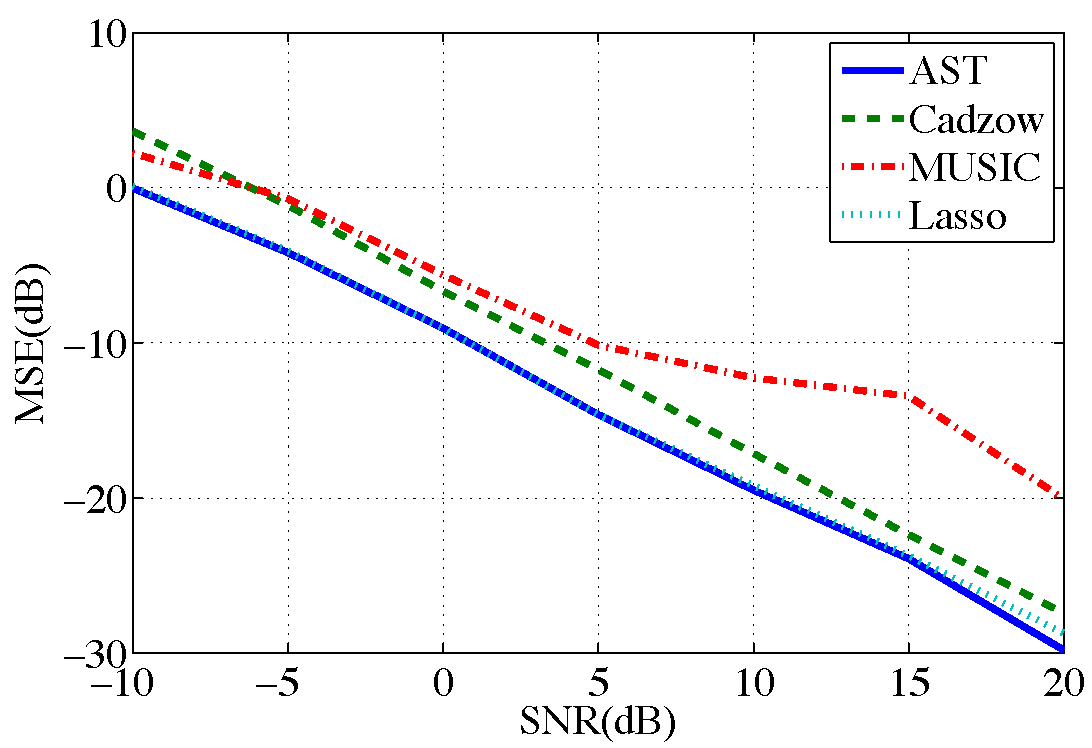
\includegraphics[width=0.5\textwidth]{figures/mse_snr_128_8_randamp}
	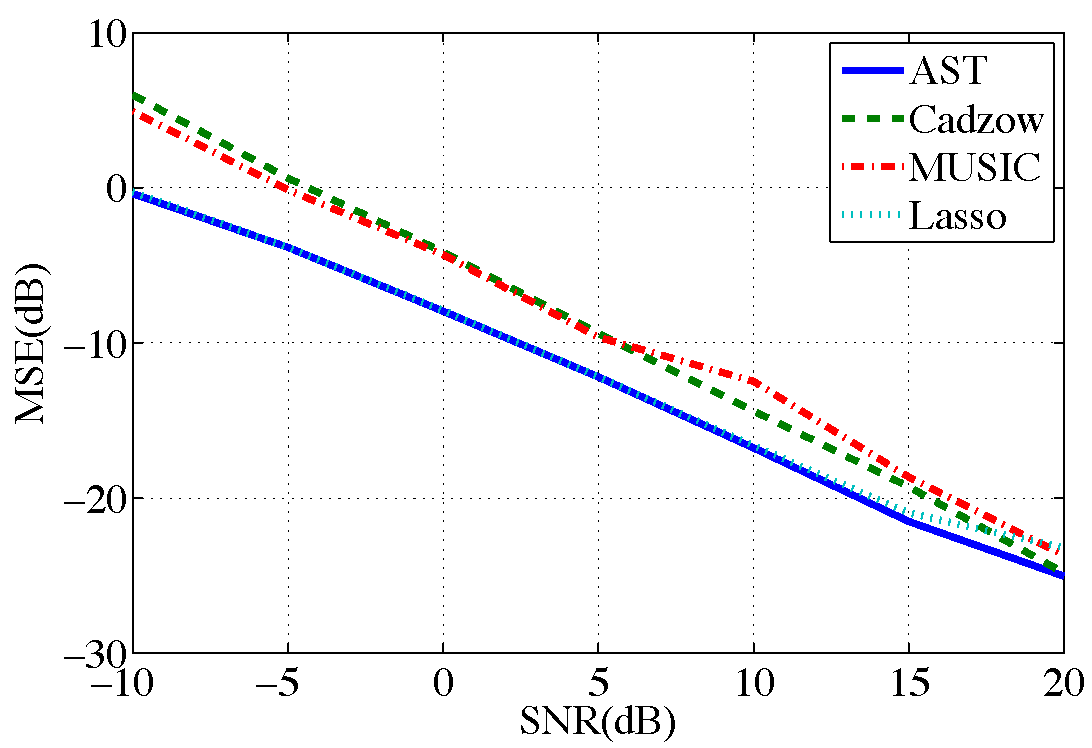
\includegraphics[width=0.5\textwidth]{figures/mse_snr_128_16_randamp} \\
	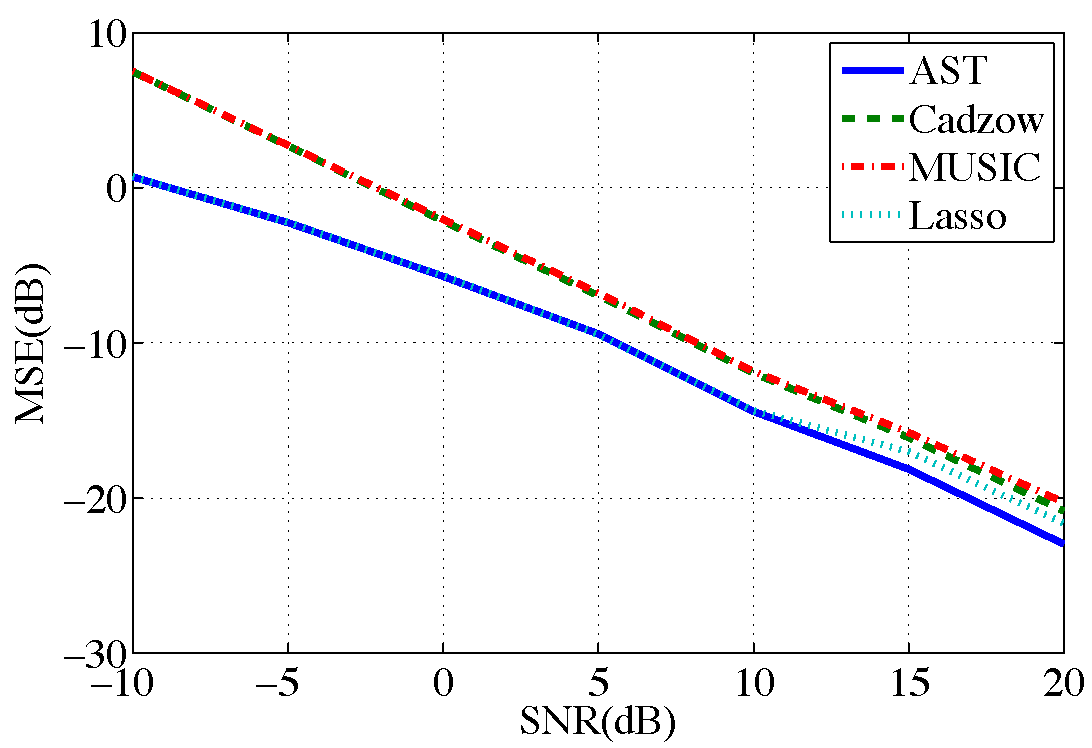
\includegraphics[width=0.5\textwidth]{figures/mse_snr_128_32_randamp}
\end{tabular}
\caption{ {\bfseries MSE vs SNR plots:} This graph compares MSE vs SNR for a subset of experiments with $n=128$ samples. From top left, clockwise, the plots are for combinations of $8$, $16$, and $32$ sinusoids with amplitudes and frequencies sampled at random.}
\label{fig:mse-snr}
\end{figure*}

In Figure~\ref{fig:mse-snr}, we show MSE vs SNR plots for a subset of
experiments when $n=128$ time samples are taken to take a closer look at the
differences. It can be seen from these plots that the performance difference
between classical algorithms such as MUSIC and Cadzow with respect to the
convex optimization based AST and Lasso is most pronounced at lower sparsity
levels. When the noise dominates the signal (SNR $\leq 0$ dB), all the
algorithms are comparable. However, AST and Lasso outperform the other
algorithms in almost every regime.


\begin{figure}[htbp]
  \begin{tabular}{cc}
	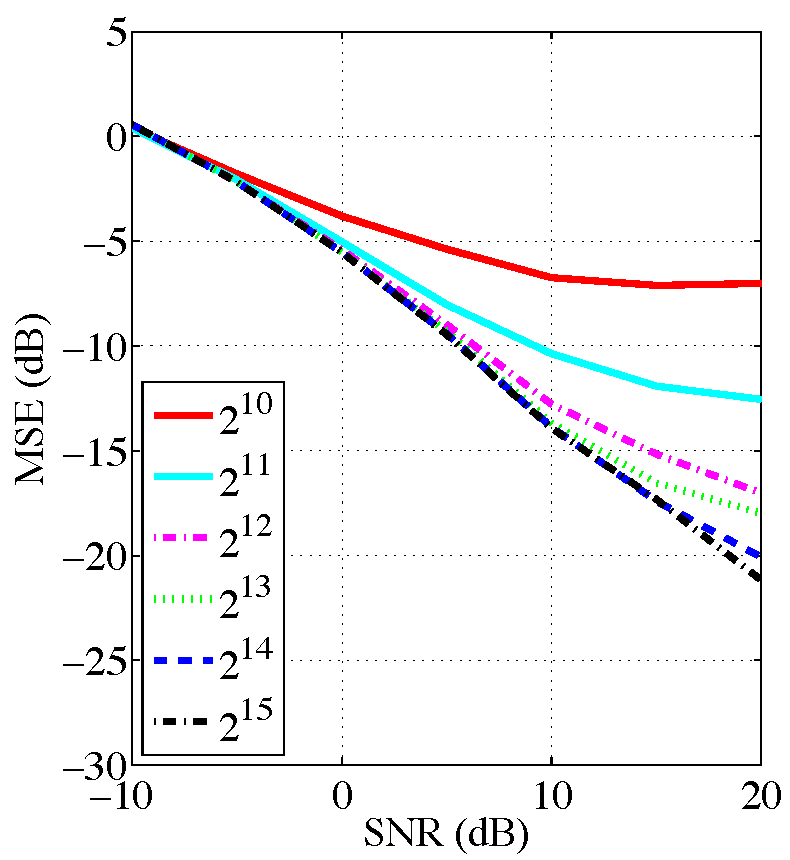
\includegraphics[trim=10mm 0mm 5mm 3mm,clip,width=0.37\linewidth]{figures/mse_snr_256_64_lasso_randamp} &
	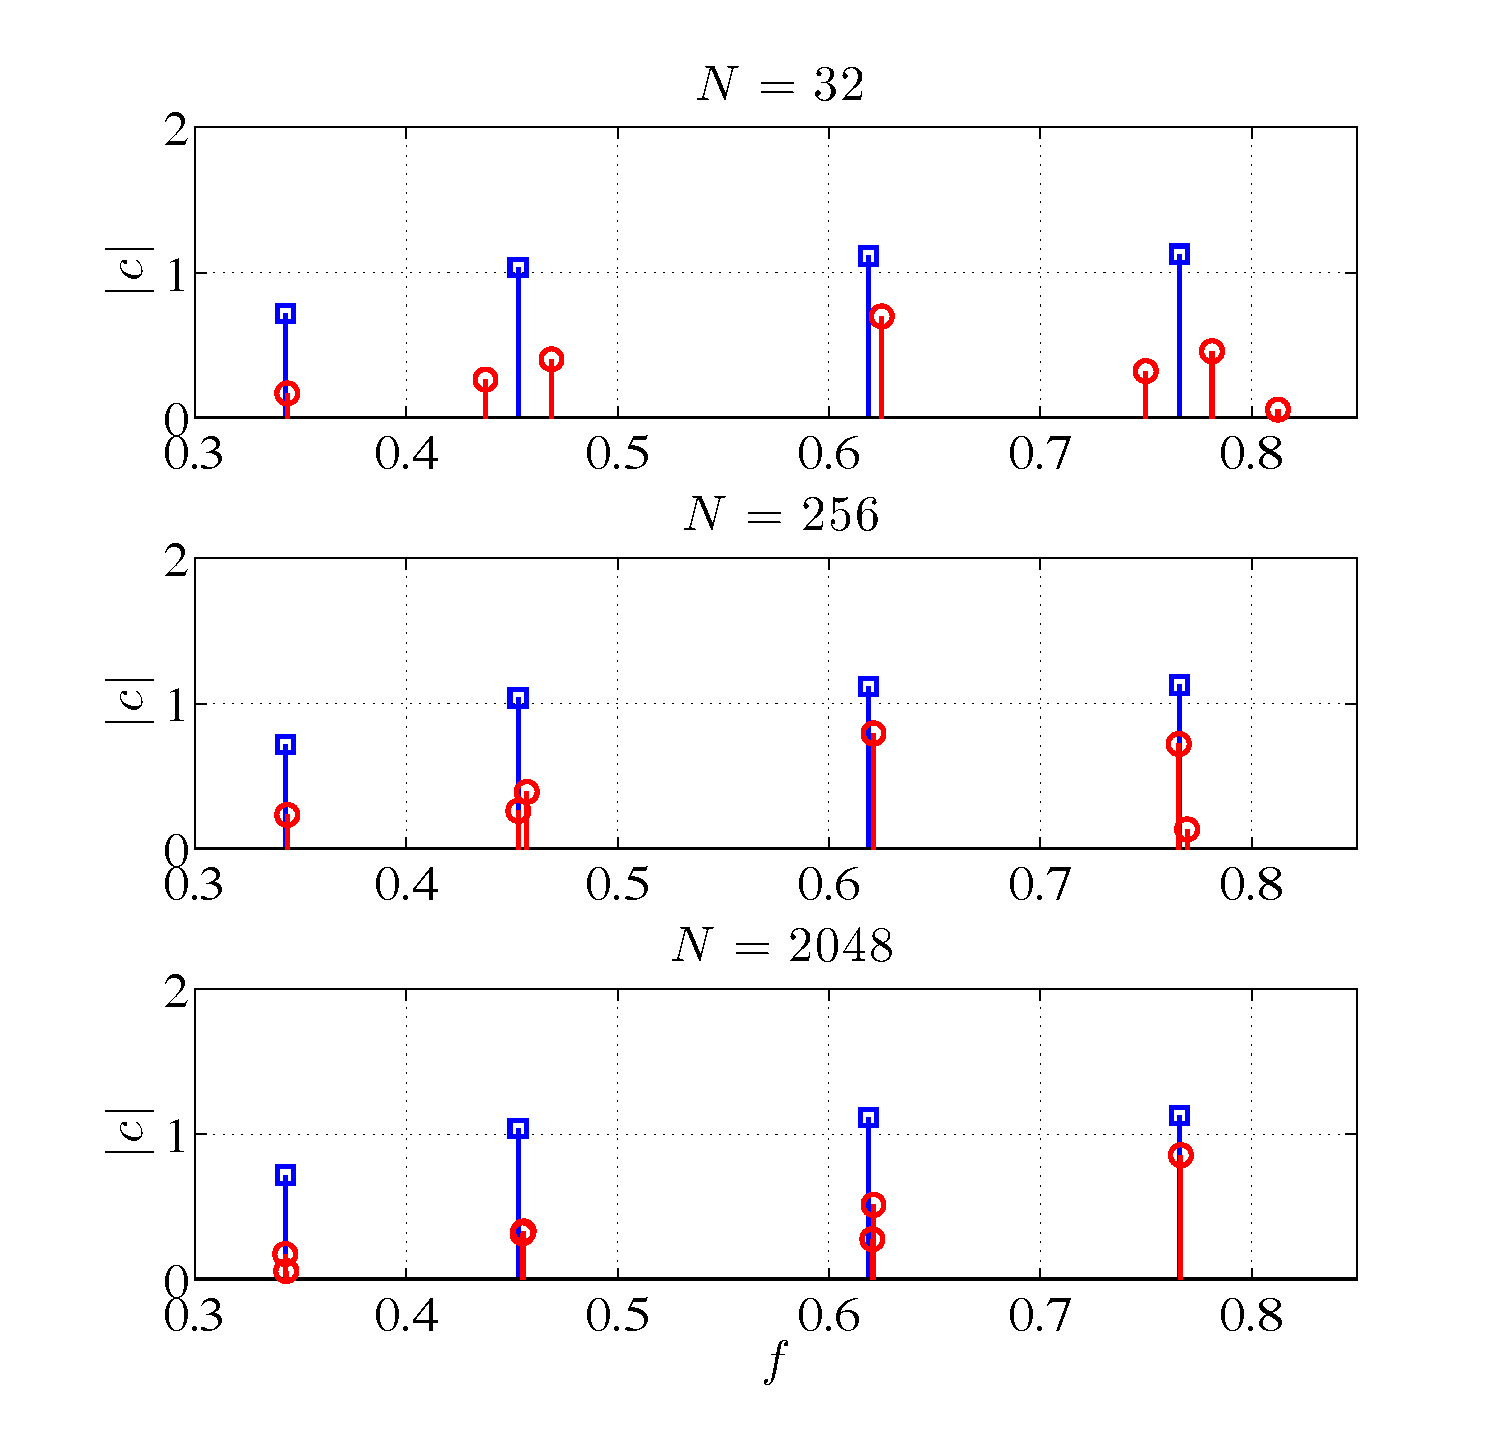
\includegraphics[trim=15mm 0mm 20mm 3mm,clip,width=0.45\linewidth]{figures/gridding} \\
(a)  & (b)
\end{tabular}
\caption{ 
(a) Plot of MSE vs SNR for Lasso at different grid sizes for a subset of experiments with $n=128, k = 16$\newline
(b) Lasso Frequency localization with $n=32, k = 4,$
SNR = $10$ dB. Blue represents the true frequencies, while red are given by Lasso. For better visualization, we threshold the Lasso solution by $10^{-6}$.}
\label{fig:lasso-compare}
\end{figure}

We note that the denoising performance of Lasso improves with increased grid
size as shown in the MSE vs SNR plot in Figure~\ref{fig:lasso-compare}(a). The
figure shows that the performance improvement for larger grid sizes is greater
at high SNRs. This is because when the noise is small, the discretization error
is more dominant and finer gridding helps to reduce this error.
Figures~\ref{fig:lasso-compare}(a) and (b) also indicate that the benefits of
increasing discretization levels are diminishing with the grid sizes, at a
higher rate in the low SNR regime, suggesting a tradeoff among grid size,
accuracy, and computational complexity.

Finally, in Figure \ref{fig:lasso-compare}(b), we provide numerical evidence
supporting the assertion that frequency localization improves with increasing
grid size. Lasso identifies more frequencies than the true ones due to basis
mismatch. However, these frequencies cluster around the true ones, and more
importantly, finer discretization improves clustering, suggesting
over-discretization coupled with clustering and peak detection as a means for
frequency localization for Lasso. This observation does not contradict the
results of \cite{cpsc} where the authors look at the full Fourier basis ($N=n$)
and the noise-free case. This is the situation where discretization effect is
most prominent. We instead look at the scenario where $N \gg n$.

In Figure~\ref{fig:msnr}, we display how the error metrics vary with
increasing SNR for AST, MUSIC and Cadzow.  We restrict these plots to the experiments with $n =
256$ samples. These plots demonstrate that AST localizes frequencies
substantially better than MUSIC and Cadzow even for low signal to noise ratios
as there is very little energy in the far region of the frequencies ($m_1$) and
has the smallest weighted mean square frequency deviation ($m_2$). Although we
have plotted the average value in these plots, we observed spikes in the plots
for Cadzow's algorithm as the average is dominated by the worst performing
instances.  These large errors are due to the numerical instability of polynomial root finding. 

\begin{figure}[htbp]
\begin{tabular}{ccc}
	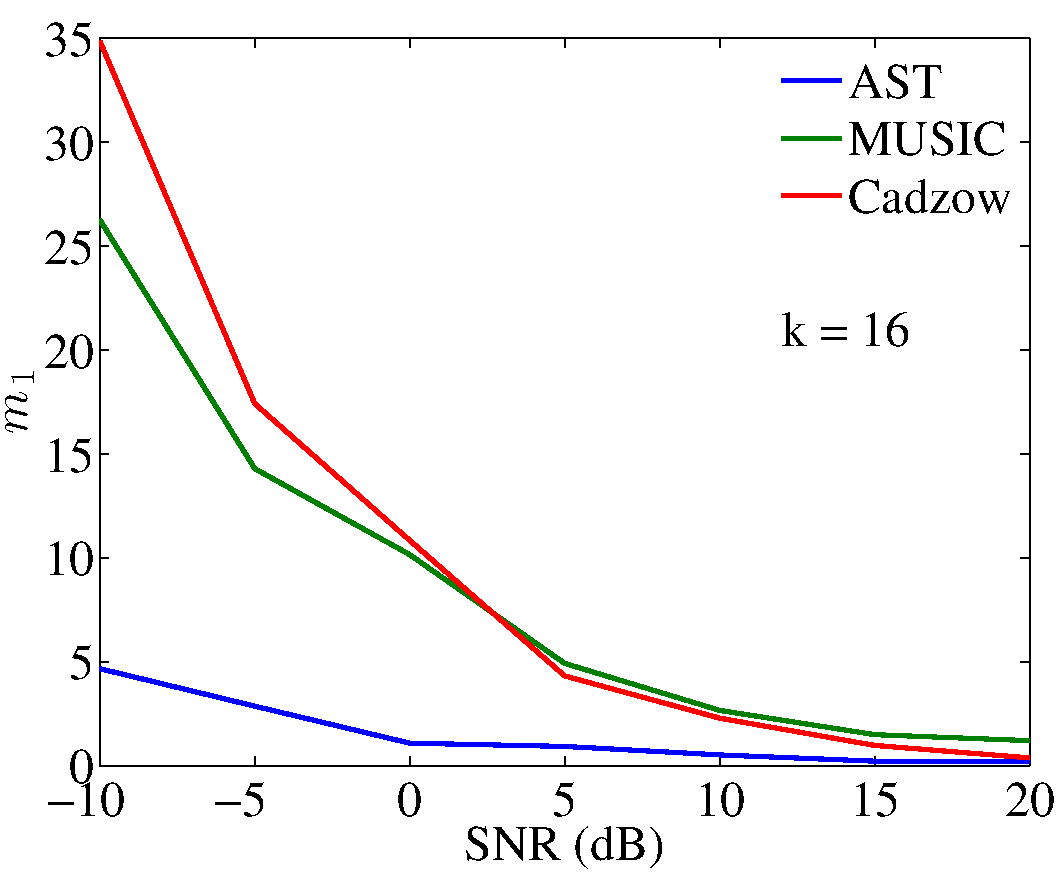
\includegraphics[height=35mm]{figures/mSNR1_16.pdf} &
	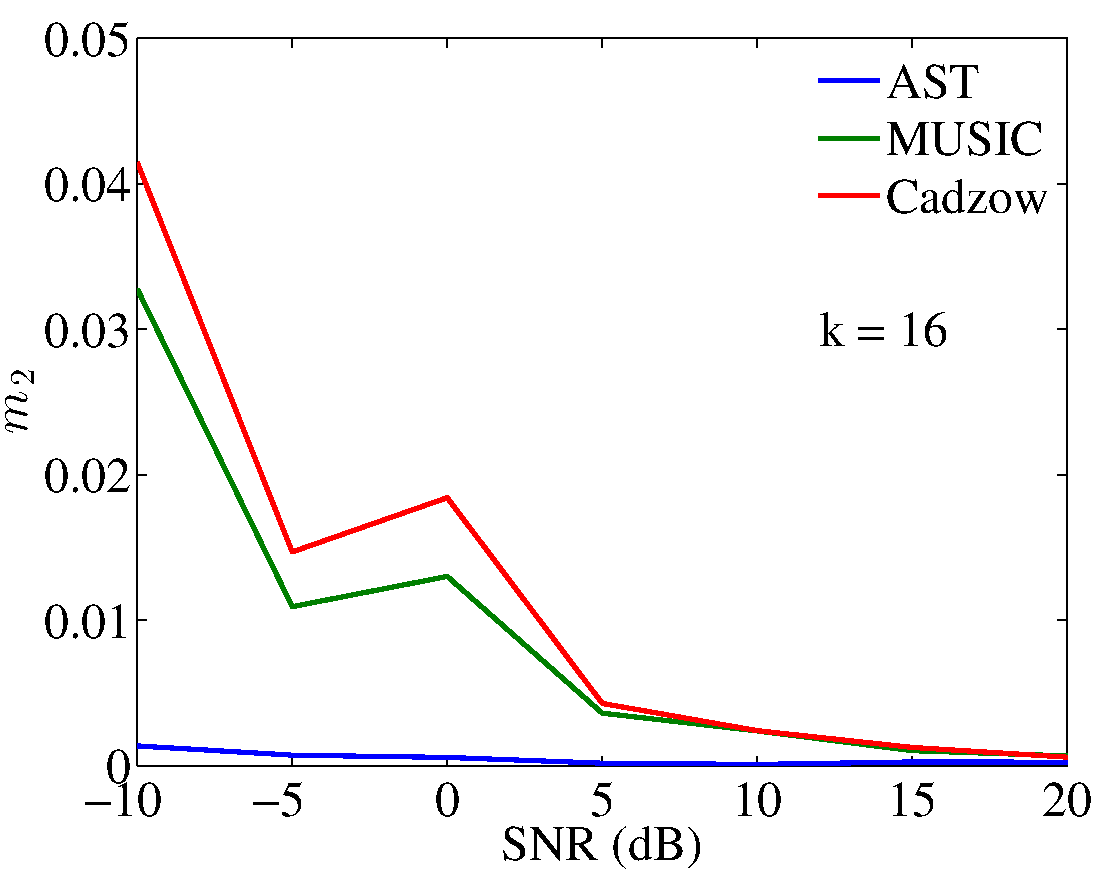
\includegraphics[height=35mm]{figures/mSNR2_16.pdf} &
	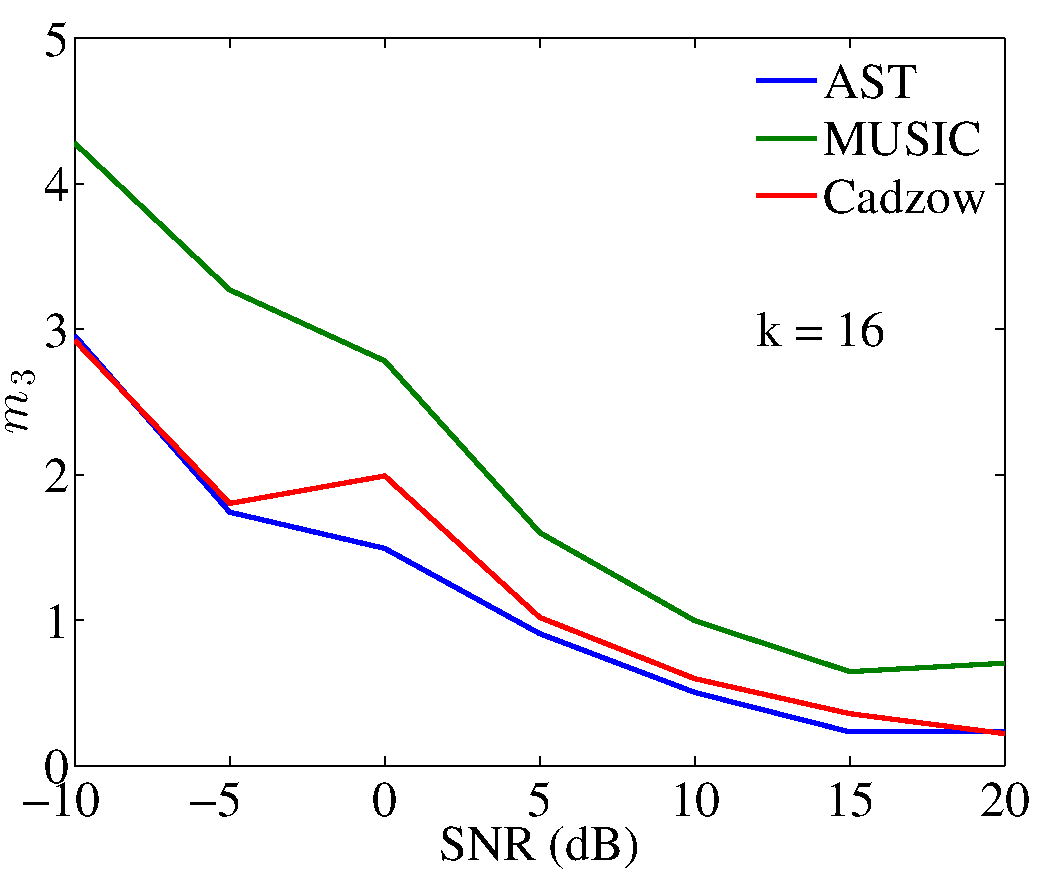
\includegraphics[height=35mm]{figures/mSNR3_16.pdf} \\
	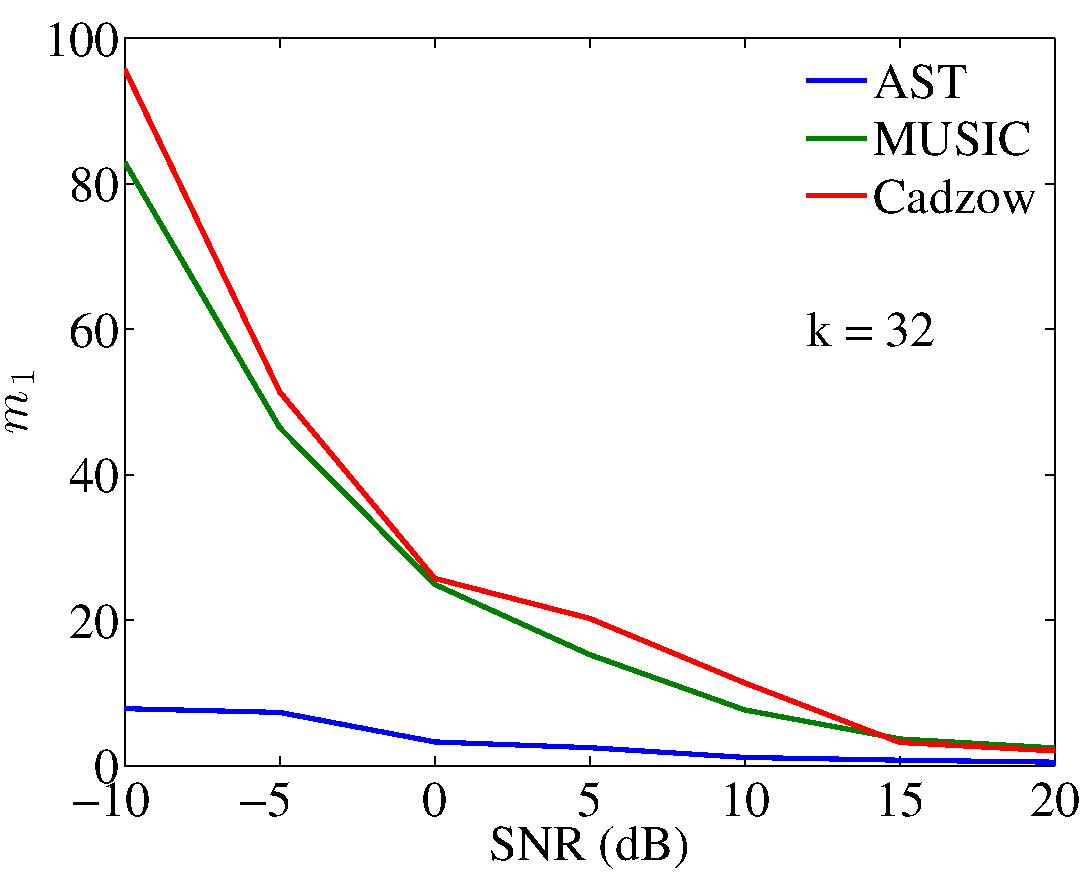
\includegraphics[height=35mm]{figures/mSNR1_32.pdf} &
	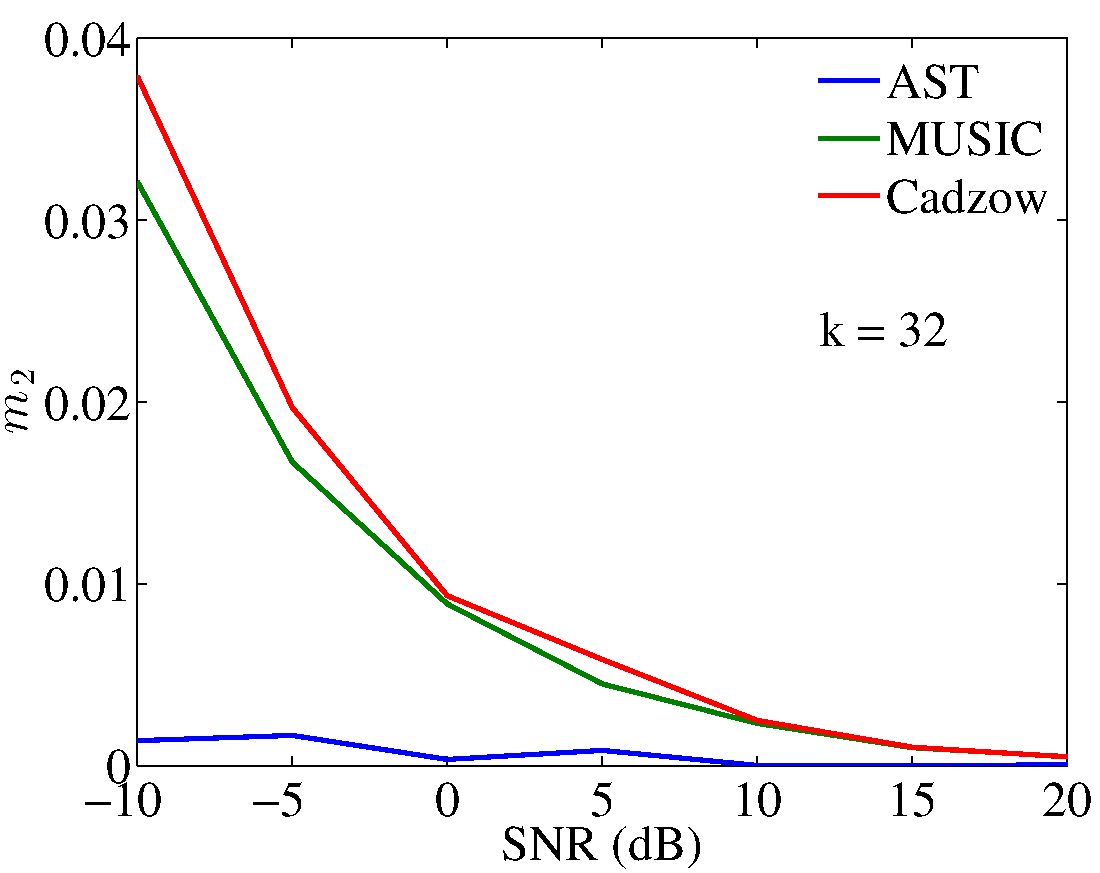
\includegraphics[height=35mm]{figures/mSNR2_32.pdf} &
	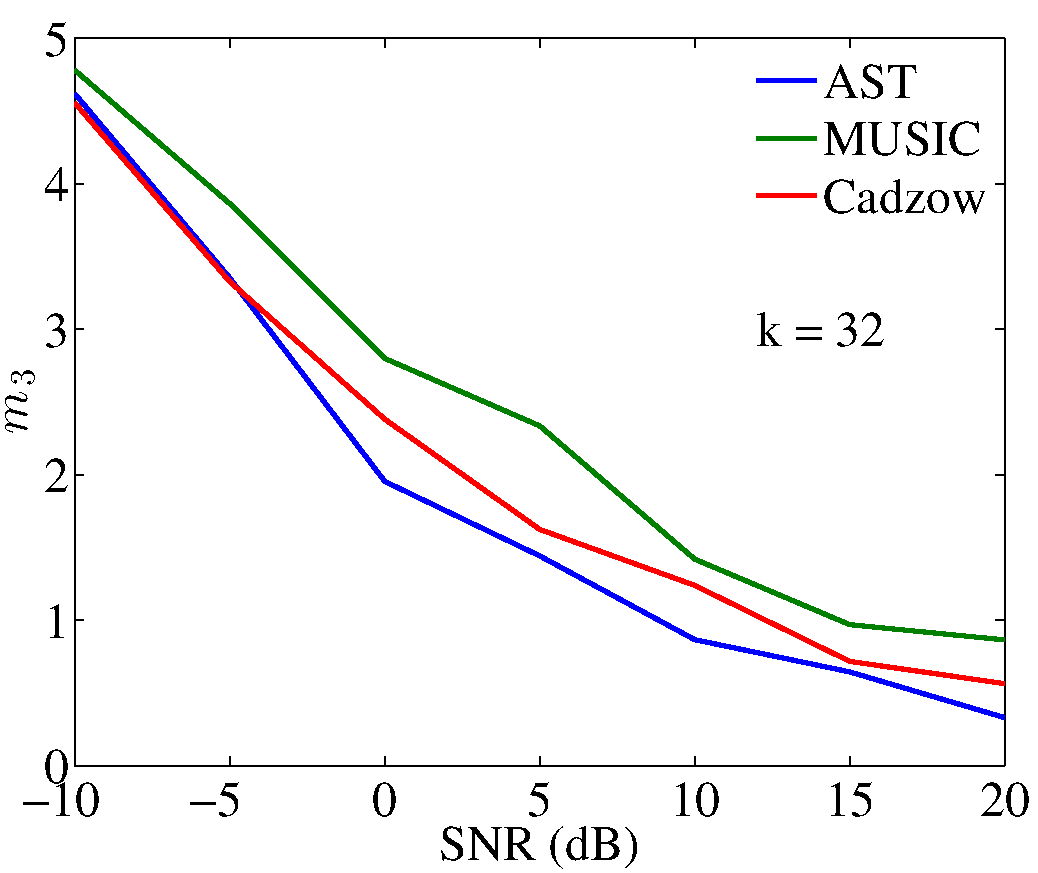
\includegraphics[height=35mm]{figures/mSNR3_32.pdf} \\
	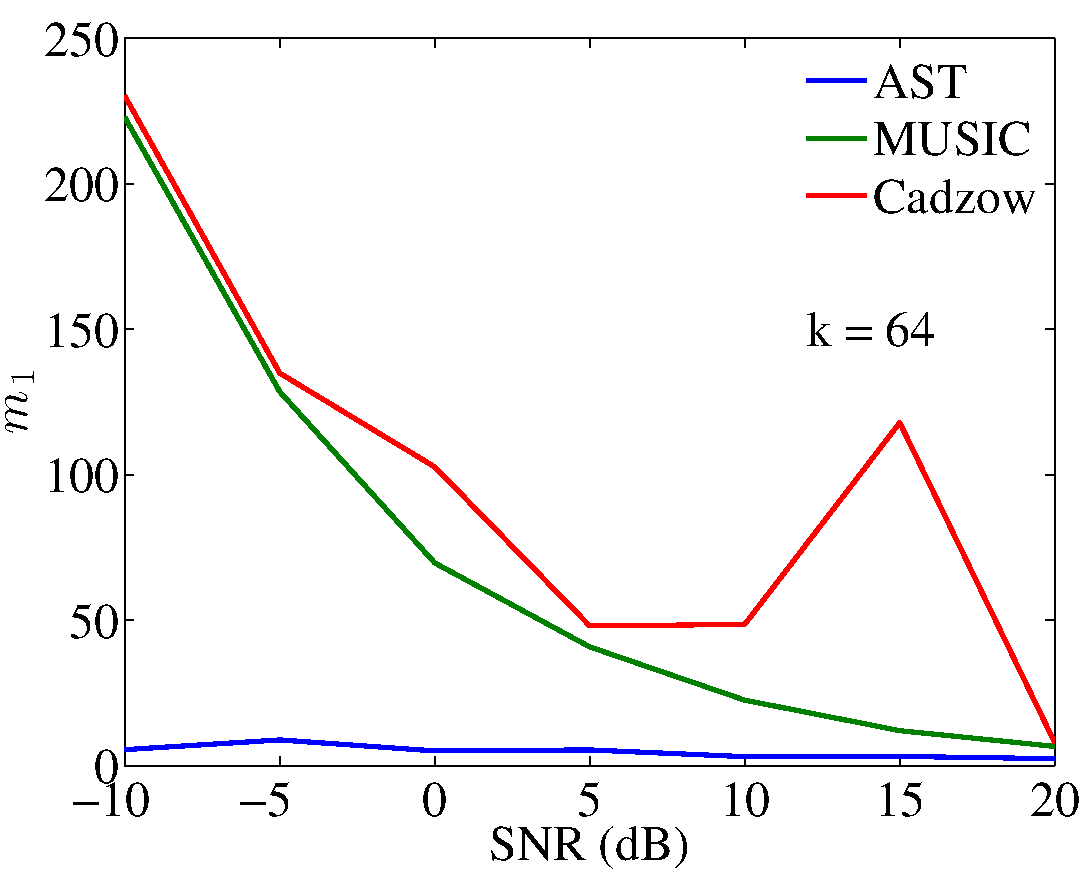
\includegraphics[height=35mm]{figures/mSNR1_64.pdf} &
	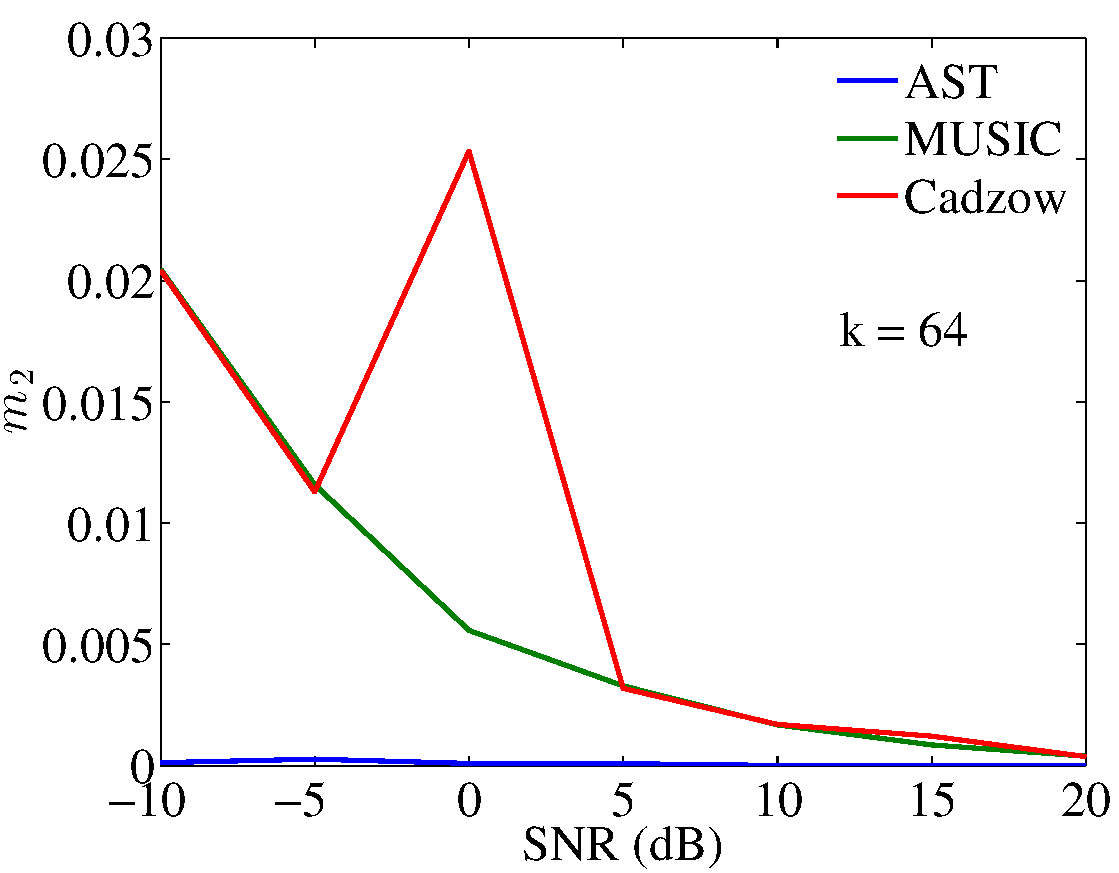
\includegraphics[height=35mm]{figures/mSNR2_64.pdf} &
	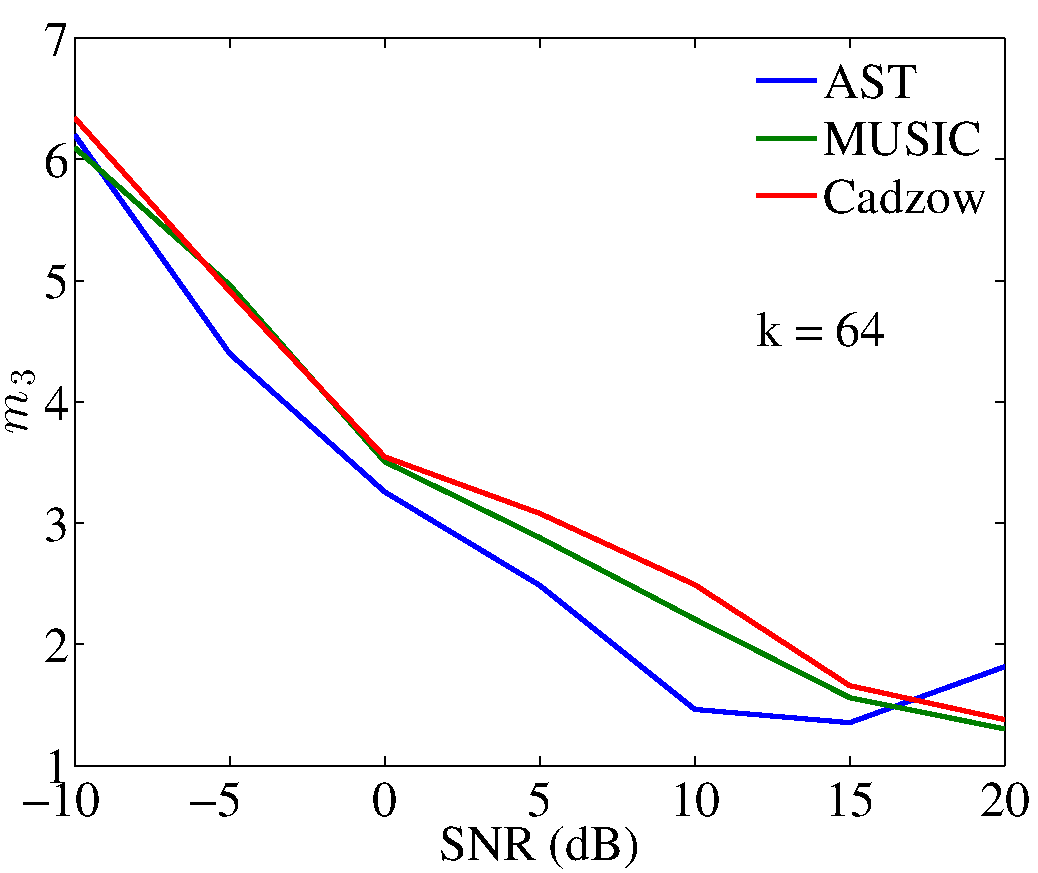
\includegraphics[height=35mm]{figures/mSNR3_64.pdf}
\end{tabular}
\caption{For $n = 256$ samples, the plots from left to right in order measure the average value over 20 random experiments for the error metrics $m_1, m_2$ and $m_3$ respectively. The top, middle and the bottom third of the plots respectively represent the subset of the experiments
with the number of frequencies $k=16, 32$ and $64$.}
\label{fig:msnr}
\end{figure}


We use \emph{performance profiles} to summarize the behavior of the various
algorithms across all of the parameter settings. Performance profiles provide a
good visual indicator of the relative performance of many algorithms under a
variety of experimental conditions\cite{dolanmore02}. Let $\mathcal{P}$ be the
set of experiments and let $\mathrm{MSE}_s(p)$ be the MSE of experiment $p \in
\mathcal{P}$ using the algorithm $s$. Then the ordinate $P_s(\beta)$ of the
graph at $\beta$ specifies the fraction of experiments where the ratio of the
MSE of the algorithm $s$ to the minimum MSE across all algorithms for the given
experiment is less than $\beta$, i.e.,

\begin{equation*}
P_s(\beta) = \frac{\mathop{\#}\left\{p \in \mathcal{P} ~:~ \mathrm{MSE}_s(p) \leq \beta \min_s \mathrm{MSE}_s(p)\right\}}{\mathop{\#}(\mathcal{P})}
\end{equation*}

\begin{figure}[htp]
\centering
\begin{tabular}{cc}
	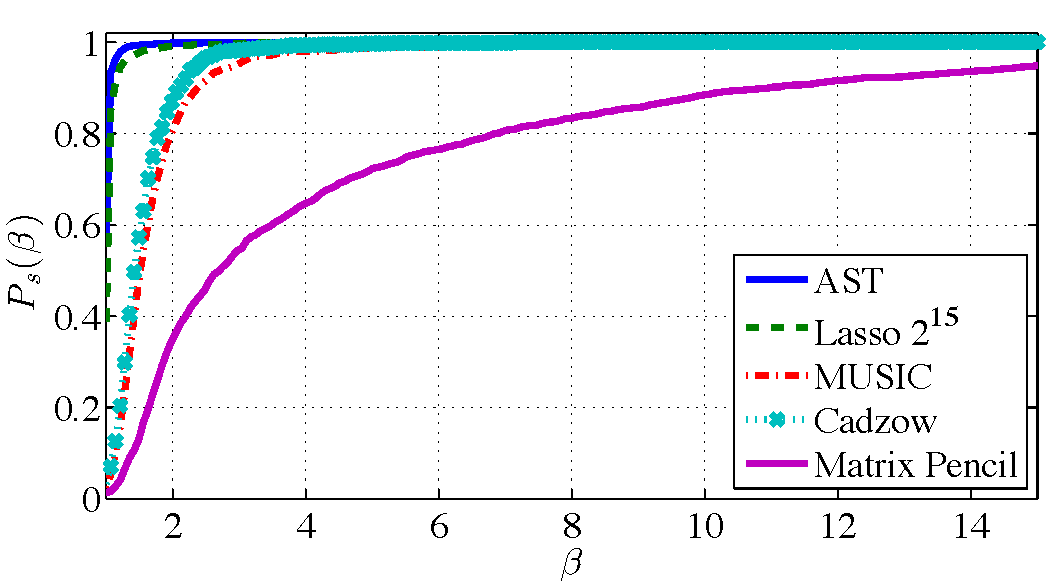
\includegraphics[height=40mm]{figures/performance_profile_randamp_color} &
	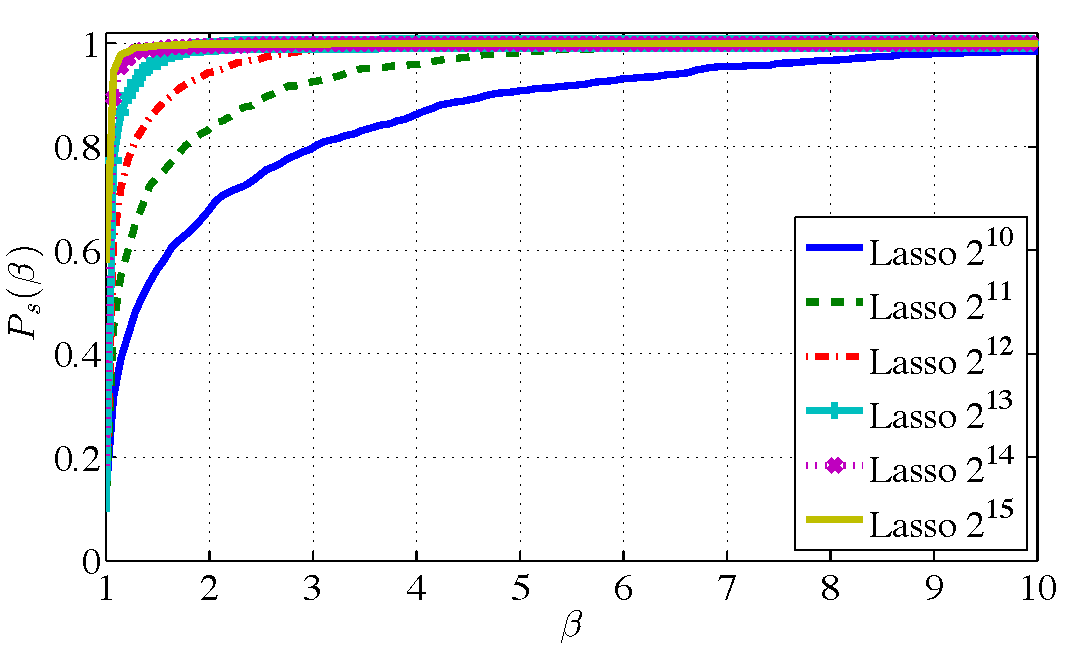
\includegraphics[trim=0mm 0mm 2mm 5mm,clip,height=40mm]{figures/performance_profile_lasso_randamp_color}\\
(a) & (b)
\end{tabular}
\caption{ (a) Performance Profile  comparing various algorithms and AST. (b) Performance profiles for Lasso with different grid sizes.}
\label{fig:pp1}
\end{figure}


From the performance profile in Figure~\ref{fig:pp1}(a), we see that AST is the
best performing algorithm, with Lasso coming in
second. Cadzow does not perform as well as AST, even though it is fed the true
number of sinusoids. When Cadzow is fed an incorrect $k$, even off by $1$, the
performance degrades drastically, and never provides adequate mean-squared
error. Figure~\ref{fig:pp1}(b) shows that the denoising performance
improves  with grid size.

\begin{figure}[htp]
\begin{tabular}{ccc}
	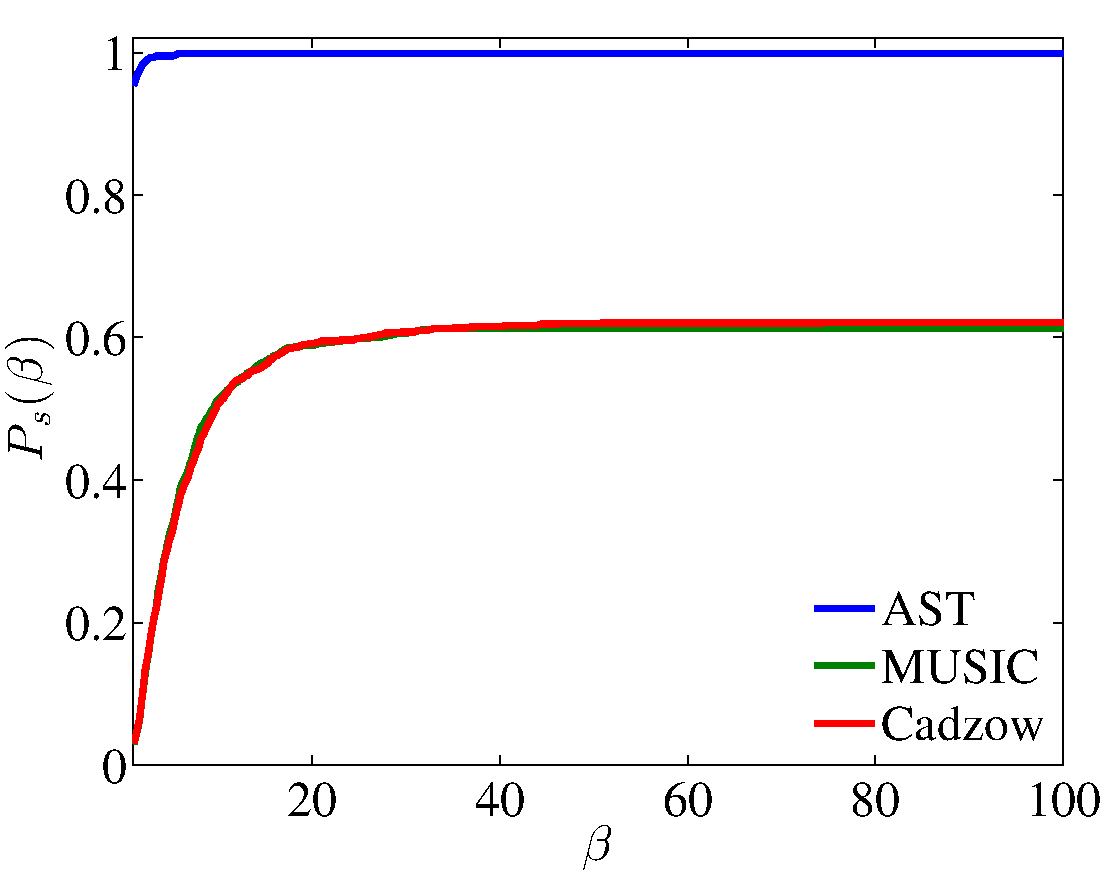
\includegraphics[height=35mm]{figures/m1_pp.pdf} &
	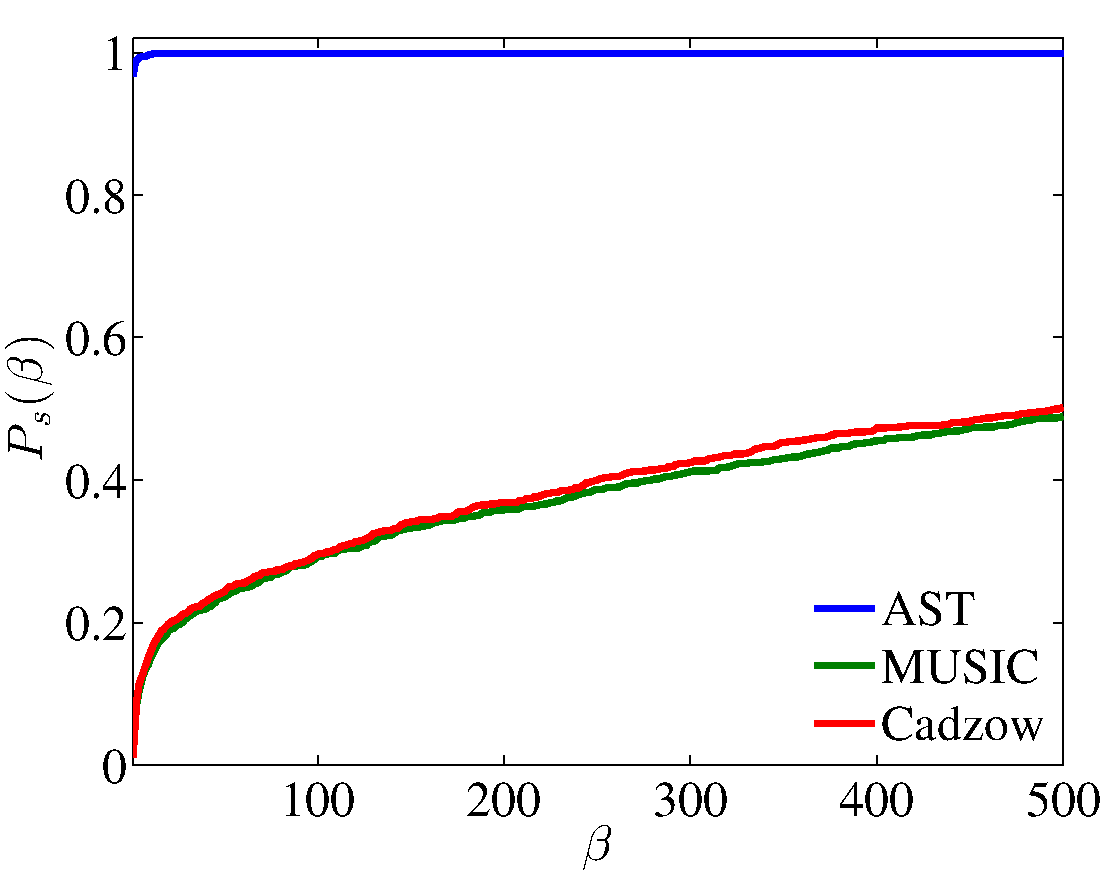
\includegraphics[height=35mm]{figures/m2_pp.pdf} &
	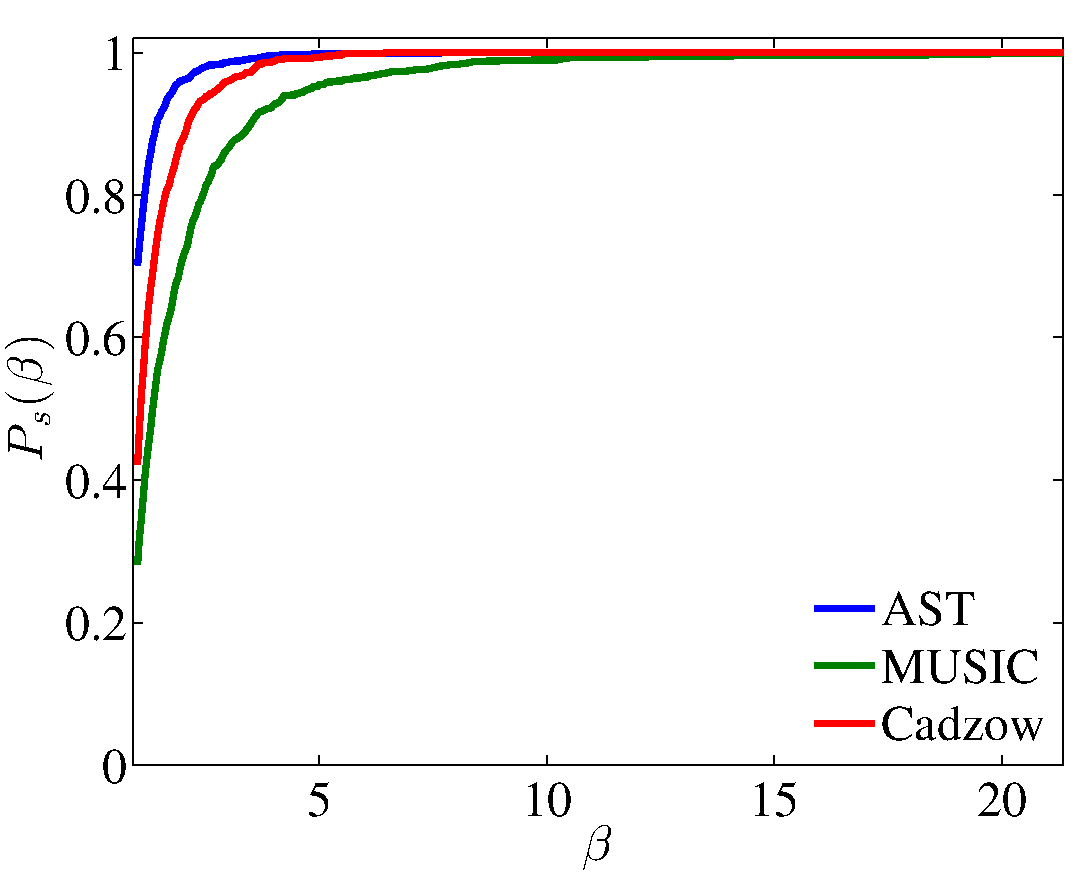
\includegraphics[height=35mm]{figures/m3_pp.pdf}\\
	(a) $m_1$ & (b) $m_2$ & (c) $m_3$
\end{tabular}
\caption{ Performance Profiles for AST, MUSIC and Cadzow.
(a) Sum of the absolute value of amplitudes in the far region ($m_1$)
(b) The weighted frequency localization error, $m_2$
(c) Error in approximation of amplitudes in the near region, $m_3$ }
\label{fig:pp2}
\end{figure}

The performance profiles in Figure~\ref{fig:pp2} show that AST is the best
performing algorithm for all the three metrics for frequency localization. AST
in fact outperforms MUSIC and Cadzow by a substantial margin for metrics $m_1$
and $m_2$.

% section ast:experiments (end)